% WSCG sample document 
%
% based on Gabriel Zachmann's sample
% http://zach.in.tu-clausthal.de/latex/
%
% modified Apr 2012 to match WSCG Word template
%
\documentclass[twoside,twocolumn,10pt]{article}
%\documentclass[twoside,twocolumn,draft]{article}

%  for debugging
%\tracingall%\tracingonline=0
%\tracingparagraphs
%\tracingpages

\usepackage{biblatex}
\usepackage[utf8]{inputenc}
\usepackage{amsmath}
\addbibresource{references.bib}

\usepackage{subfig}




%%%%%%%%%%%%%%%%%%%%%%%%%%%%%%%%%%%%%%%%%%%%%%%%%%%%%%%%%%%%%%%%%%%%%%%%%%%%%
%                             Packages

\usepackage{wscg}           % includes a number of other packages (e.g., myalgorithm)
\RequirePackage{ifpdf}
\ifpdf
 \RequirePackage[pdftex]{graphicx}
 \RequirePackage[pdftex]{color}
 
\else
 \RequirePackage[dvips,draft]{graphicx}
 \RequirePackage[dvips]{color}
\fi
%\usepackage[german,english]{babel}     % default = english
%\usepackage{mypicture}      % loads graphicx.sty, color.sty, eepic.sty
%\usepackage{array}          % better tabular's & arrays, plus math tabular's
%\usepackage{tabularx}      % for selfadjusting p-columns
%\setlength{\extrarowheight}{1ex}   % additional space between rows
%\usepackage{booktabs}      % typographically much better
%\usepackage{mdwlist}        % for compacted lists, and more versatile lists
%\usepackage[intlimits]{amsmath} % more math stuff, see texdoc amsldoc
%\usepackage{mymath}         % own commands, loads amssymb & array.sty
%\usepackage{hyphenat}      % hyphenatable -, /, etc.
%\usepackage{theorem}
%\usepackage[sort&compress]{natbib}% better \cite commands, more flexible
%\usepackage[sort&compress,super]{natbib} % better \cite commands, more flexible
%\newcommand{\citenumfont}[1]{\textit{#1}}


\usepackage{nopageno}       % no page numbers at all; uncomment for final version
\usepackage{bm} 
\usepackage{amsmath,amsfonts,amssymb}

\usepackage{todonotes}

%%%%%%%%%%%%%%%%%%%%%%%%%%%%%%%%%%%%%%%%%%%%%%%%%%%%%%%%%%%%%%%%%%%%%%%%%%%%%
%                                Title


\title{Fast triangle-based glyph rendering scheme for high angular resolution diffusion imaging}

\author{
\parbox{0.25\textwidth}{\centering
Daniel Silva\\[1mm]
DCA/FEEC/University of Campinas,\\
%1st line of address\\
%2nd line of address\\
Brazil\\[1mm]
danielxs@dca.fee.unicamp.br
}
\hspace{0.05\textwidth}
\parbox{0.25\textwidth}{\centering
Second Author\\[1mm]
author's affiliation\\
1st line of address\\
2nd line of address\\
Country (ZIP) code, City, State\\[1mm]
e@mail
}
\hspace{0.05\textwidth}
\parbox{0.25\textwidth}{\centering
Third Author\\[1mm]
author's affiliation\\
1st line of address\\
2nd line of address\\
Country (ZIP) code, City, State\\[1mm]
e@mail
}
}

%%%%%%%%%%%%%%%%%%%%%%%%%%%%%%%%%%%%%%%%%%%%%%%%%%%%%%%%%%%%%%%%%%%%%%%%%%%%%
%                          Hyperref


% no hyperlinks
\usepackage{url}
\urlstyle{tt}

% Donald Arsenau's fix for missing kerning of "//" and ":/"
\makeatletter
\def\Uslash{\mathbin{\mathchar`\/}\@ifnextchar{/}{\kern-.15em}{}}
\g@addto@macro\UrlSpecials{\do \/ {\Uslash}}
\def\Ucolon{\mathbin{\mathchar`:}\@ifnextchar{/}{\kern-.1em}{}}
\g@addto@macro\UrlSpecials{\do : {\Ucolon}}
\makeatother

%added by Ting
\usepackage[normalem]{ulem}
\usepackage{todonotes}

%%%%%%%%%%%%%%%%%%%%%%%%%%%%%%%%%%%%%%%%%%%%%%%%%%%%%%%%%%%%%%%%%%%%%%%%%%%%%
%                              My Commands


%\DeclareMathOperator{\sgn}{sgn}

%\theorembodyfont{\upshape}
%\theoremstyle{break}
%\theoremheaderfont{\bfseries\normalsize}

%\newtheorem{lem}{Lemma}
%\newtheorem{defn}{Definition}

%%%%%%%%%%%%%%%%%%%%%%%%%%%%%%%%%%%%%%%%%%%%%%%%%%%%%%%%%%%%%%%%%%%%%%%%%%%%%
%                                Document


\begin{document}

\twocolumn[{\csname @twocolumnfalse\endcsname

\maketitle  % full width title


\begin{abstract}
\noindent

Diffusion magnetic resonance imaging provides the quantification of the diffusion process of water molecules. Applied to the brain, it is unique in providing white matter fiber structures and connectivity in-vivo, relying on the fact that the water molecules' displacements are greater along with the fiber orientation than perpendicular to it due to biological barriers. For reconstructing multiple fibers passing through the same voxel, high angular resolution diffusion imaging (HARDI) acquisition scheme has been introduced. Advanced methods for processing diffusion data were developed to synthesize HARDI data into orientation distribution functions (ODF), consisting of an association between directions and probabilities of water diffusion along with these directions on the sphere. Visualizing ODFs helps in gaining insight into the local structure of the brain white matter. In this work, we present an interactive GPU triangle-based rendering scheme for ODF. We show how the advanced GPU features may be exploited to make the triangle-based rendering competitive with the ray-casting one, despite ODF data's high dimensionality. Performance measurements are presented to demonstrate the proposed GPU-based rendering algorithm's interactivity.


%We describe the formatting guidelines for the Journal of WSCG and WSCG proceedings adapted from the ACM and SIGGRAPH proceedings and recent WSCG templates.  Please, try to fix format of your contribution as close as possible if you use other tools.

\end{abstract}

\subsection*{Keywords}
%Keywords are your own designated keywords - Times New Roman, 10pts.
medical visualization, HARDI, computer graphics, visualization. 

\vspace*{1.0\baselineskip}
}]

\todo[inline]{Is ODF a representation of HARDI data or a representation of a HARDI data processing tool?}

\todo[inline]{In our approach ... you should }

%%%%%%%%%%%%%%%%%%%%%%%%%%%%%%%%%%%%%%%%%%%%%%%%%%%%%%%%%%%%%%%%%%%%%%%%%%%%%
\section{Introduction}

\copyrightspace

Diffusion-weighted magnetic resonance imaging (DWI) is a technique that aims to measure the random Brownian motion of water molecules. Applied to the brain, it is unique in providing in-vivo information on the white matter path. Imaging methods to synthesize the diffusion signals into functions have been a research subject for more than two decades.

The first and the most applied method in the clinical area is diffusion tensor imaging (DTI) \cite{Basser1994}. The technique aims to fit a set of diffusion signal samples into a Gaussian 3D model.
%%, of average zero, and the diffusion tensor is the covariance matrix.
This fitting works  well for the diffusion behavior in points that have only one underlying fiber. However, it fails to model regions with multiple fibers and more complex behavior (i.e., fiber crossing, branching, kissing, merging, and fanning). This limitation critically affects the reconstruction accuracy of the underlying fiber \cite{descoteaux2015,SCHILLING2019194}.

%The limitations of DTI are well known \cite{descoteaux2015,SCHILLING2019194}. The \sout{gaussian assumption}\textcolor{blue}{Gaussian distribution} fits well the diffusion behavior when the point represents a \textcolor{blue}{brain} region \sout{of the brain} that \textcolor{blue}{only} one fiber passes through it\sout{, but}\textcolor{blue}{But,} the model is limited when \sout{it comes to describe}\textcolor{blue}{describing} the diffusion in areas \sout{that have}\textcolor{blue}{with} fibers \sout{with a}\textcolor{blue}{of} more complex behavior (\sout{ie.}\textcolor{blue}{i.e.,} fiber crossing, branching, kissing). This limitation \sout{affects} critically \textcolor{blue}{affects} the accuracy \sout{on}\textcolor{blue}{of} inferring the fiber distribution in the brain.

High angular resolution diffusion imaging (HARDI) acquisitions and more advanced methods for processing diffusion data, such as Q-Ball imaging \cite{TuchQBall2004} and constrained spherical deconvolution \cite{tournier2007}, were introduced to overcome the Gaussian model's limitation \cite{descoteaux2015}. These methods are typically represented as an orientation distribution function (ODF) $\psi(\bm{u})$, which consists of an association of a set of unit directional vectors to diffusivity scalars. %These methods require more samples on the DWI acquisitions than those applied on DTI. %These acquisitions are called High Angular Resolution Diffusion Imaging (HARDI). While the amount of diffusion-weighted acquisitions used on DTI vary between 6 and 32, HARDI acquisitions have more than 45 .
%\sout{To overcome the limitation of the gaussian model assumption, m}\textcolor{blue}{M}ore advanced imaging methods for diffusion were introduced \textcolor{blue}{to overcome the limitation of the Gaussian model}. These methods require more samples on the DWI \textcolor{blue}{acquisitions} than \textcolor{blue}{those applied } \sout{the acquisitions used} on DTI\sout{ and t}\textcolor{blue}{. T}hese acquisitions \sout{were labeled as}\textcolor{blue}{are called} High Angular Resolution Diffusion Imaging (HARDI). While the amount of diffusion-weighted acquisitions used on DTI vary between 6 and \todo{For very special cases ...}32, HARDI acquisitions have \todo{In competitions less number of acquisitions were applied ...}more than 45 \cite{descoteaux2015}.
%\sout{The most common method to visualize HARDI data through the\sout{se} advanced imaging methods is \sout{by} spherical polar plot\textcolor{blue}{s or HARDI} glyphs. These methods}
%HARDI data are typically pre-processed into a model-free orientation distribution function (ODF) $\psi(\bm{u})$, which consist\sout{s} \sout{of}\textcolor{blue}{in} an association of a set of \sout{directions, represented by} unit \textcolor{blue}{directional} vectors\sout{,} to \sout{scalars representing the corresponding} diffusivity \textcolor{blue}{scalars. \todo{Use consistently one name.}The most common method to visualize ODFs is spherical polar plots, also known as HARDI glyphs and ODF glyphs}\sout{for each element in the domain}. 


% for all $\bm{u} \in \mathbb{R}^3 and |\bm{u}| = 1$

The most common method to visualize ODF data is through glyphs generated by its respective spherical polar plot $R(\bm{u})=\psi (\bm{u})$. It is useful to generate the glyphs using the min-max normalized version of the ODF \cite{TuchQBall2004} to emphasize the dominant diffusion directions. Eq. \ref{eq::normglifo} presents the magnitude of each vector $\bm{u}$ after the min-max normalization of $\psi(\bm{u})$ at the point $\bm{u}$ on the sphere. In this work, we call the spherical polar plot of a min-max normalized ODF as ODF glyphs.

\begin{figure}[htb]
    \centering
    %\rule{6cm}{3cm}
    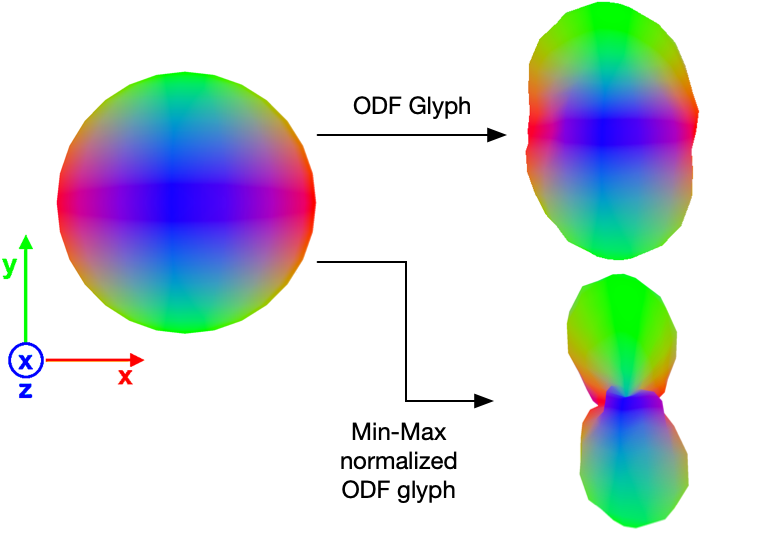
\includegraphics[width=.45\linewidth, angle=0]{figs/SphericalMeshModulation.png}
    \caption{Spherical polar plots of an ODF and its respective min-max normalized version. The min-max normalized version of the ODF, has a more pronounced orientational structure. The color scheme is described in the equation \ref{eq::glyph_color}.}
    \label{fig::intro_glyph}
\end{figure}

%\sout{These advanced methods that requires a HARDI acquisition, which will be called in this work as HARDI methods, aims to reconstruct} \textcolor{blue}{Tuch showed that when the angular acquisitions are uniform, one can synthesize from the samples} an orientation distribution function (ODF) that represents the diffusion process. \sout{Some of them are}\textcolor{blue}{This function is} model-free\sout{, which}\textcolor{blue}{It} estimates the diffusion displacement from the Fourier relation between the DW-MRI signal to its respective diffusion displacement \cite{TuchQBall2004, wedeen2005,  yeh2010}\sout{ and others are}\textcolor{blue}{Tournier presented a} model-based \textcolor{blue}{approach}\todo{It is not clear the underlying model! FOD, fiber orientation density???}\textcolor{red}{, where they model the underlying fiber signal obtained by its respective decay on the diffusion acquisition \cite{tournier2007}.}

%\sout{These advanced methods that requires a HARDI acquisition, which will be called in this work as HARDI methods, aims to reconstruct} \textcolor{blue}{Tuch showed that when the angular acquisitions are uniform, one can synthesize from the samples} an orientation distribution function (ODF) that represents the diffusion process. \sout{Some of them are}\textcolor{blue}{This function is} model-free\sout{, which}\textcolor{blue}{It} estimates the diffusion displacement from the Fourier relation between the DW-MRI signal to its respective diffusion displacement \cite{TuchQBall2004, wedeen2005,  yeh2010}\sout{ and others are}\textcolor{blue}{Tournier presented a} model-based \textcolor{blue}{approach}\todo{It is not clear the underlying model! FOD, fiber orientation density???}\textcolor{red}{, where they model the underlying fiber signal obtained by its respective decay on the diffusion acquisition \cite{tournier2007}.}

%An ODF consists in an association of a set of directions, each one of \sout{them}\textcolor{blue}{which} \textcolor{blue}{is} represented by a unity vector $\bm{u}$, to a scalar $\psi(\bm{u})$. The most common approach to represent an ODF by a glyph is through the spherical polar plot. In this category of a glyph, a \todo{Reference to normalized ODF}normalized \sout{version of the} ODF deforms a sphere accordingly to \sout{the equation}\textcolor{blue}{Eq.} \ref{eq::normglifo}:

\begin{equation}
\label{eq::normglifo}
    R(\bm{u}) = \frac{\psi(\bm{u}) - min(\psi(\bm{u}))}{max(\psi(\bm{u})) - min(\psi(\bm{u}))}
\end{equation}

Fig. \ref{fig::intro_glyph} illustrates comparatively a spherical polar plot generated by an ODF with its respective min-max normalized version. Note the use of color to enhance the orientation. A simple color mapping, commonly used by the DWI community, is applied to the unit vector  $\bm{u} = (u_x, u_y, u_z)$ to get the RGB components, as defined in Eq. \ref{eq::glyph_color}.

\begin{equation}
\label{eq::glyph_color}
    r = |u_x| ~~~~ g = |u_y| ~~~~ b = |u_z|, 
\end{equation}

where, concerning anatomical planes, the red color ($r$) represents the mediolateral direction, the green ($g$) refers to the anteroposterior direction, and the blue ($b$), inferior-superior direction.

%where $R(\bm{u})$ is the length of a deformed sphere in the direction $\bm{u}$.

These glyphs provide a coherent visualization of local diffusion in each DWI sample. Researchers use them to validate imaging methods \cite{descoteaux2007_QBI,  TuchQBall2004,tournier2007,Tournier2004DirectEO, tuch2002,  yeh2010} and assess \todo{What do you mean?}\textcolor{red}{the local relationship between the acquisition quality}, imaging method, and estimation of the underlying fiber configuration \cite{cho2008, daducci2014,descoteaux2007, vega2009}. %The FODs extracted from an imaging method applied to a DWI acquisition are used as input of fiber tracking algorithms. %The conjecture of the possibility of brain connectivity from the DWI acquisitions motivates this research area's main motivation.

It is highly desirable to visualize and explore HARDI data in an interactive way. It would improve the brain connection research quality and help to move advanced diffusion imaging into clinical practice. However, the high dimensionality of ODF has been an obstacle, especially when one wants to take advantage of GPU's capacity and performance \cite{peeters2009}.

\textcolor{blue}{Peeters et al.~\cite{peeters2009} advocated that the ray-casting approach is more appropriate to deal with CPU-GPU data transfer bottleneck. The amount of data to be transferred from CPU to GPU could be greatly reduced by only passing the position and coefficients of the ODF glyph's geometric representation. Besides, in the ray-casting approach, the glyph rendering quality is not dependent on the mesh resolution as triangle-based one. However, Voltoline and Wu showed that the advanced GPU features, \todo{\textcolor{magenta}{We could be more specific on }}namely instanced rendering, transform feedback, tesselation shader, and indirect rendering, could make the triangle-based rendering competitive with the ray-casting one, with the advantage of avoiding the root-finding problem and exploring the outperformance of the triangle hardware graphics accelerator.}
%\textcolor{magenta}{In this work, we explore instance rendering }
%\todo{Insert a figure to help in understanding.}These glyphs\textcolor{blue}{, as illustrated in Fig~\ref{???},} \sout{give}\textcolor{blue}{provide} a clear visualization of local \sout{information in} diffusion \sout{imaging methods} \textcolor{blue}{in each voxel}. \sout{It is used by} \todo{References?}Researchers use them to \todo{???}\textcolor{red}{assess the acquisition quality,} \sout{attest the validity of}\textcolor{blue}{validate} an imaging method, \sout{the adequability of it given an acquisition} and \sout{the} check the relationship between the \textcolor{blue}{applied} imaging method \sout{used with} \textcolor{blue}{and the} fiber reconstruction algorithms called tractography.


%\todo[inline]{I suggest writing motivation to this work: the challenging remaining problems and the one you are supposed to solve.}

In this work, we present an interactive GPU-accelerated triangle-based rendering scheme of multiple spherical polar plots. We applied \sout{instance rendering to reduce the CPU-GPU data traffic}\textcolor{blue}{the principle of GPU-based superquadric glyphs rendering proposed by Voltoline and Wu~\cite{voltoline2021} to the spherical polar plot's rendering}.

%\sout{The gains of performance are given by decreasing the amount of data traffic CPU-GPU by taking out redundant information on each drawing request. This is achieved by using instance rendering.}

%In this work, we present a\textcolor{blue}{n interactive GPU-accelerated} rendering scheme \sout{that aims to, given samples of ODFs associated with a spherical mesh, we} \textcolor{blue}{to} render a set of spherical polar plot\textcolor{blue}{s from ODF samples}. \textcolor{blue}{Inspired by Voltoline and Wu's work, we applied instance rendering and transform feedback to reduce the CPU-GPU data traffic.}\sout{The gains of performance are given by decreasing the amount of data traffic CPU-GPU by taking out redundant information on each drawing request. This is achieved by using instance rendering.}

\todo{is rendering necessary for visualization?}\sout{This rendering scheme, integrated with visualization systems to diffusion images, can be a powerful tool for researchers in the area to assess a set of local diffusion profiles and improve their understanding of advanced methods for diffusion imaging.}

This paper is organized into \ref{sec::conclusions} sections. In Section \ref{sec::related_work}, we discuss the related works; \textcolor{blue}{in Section \ref{sec:superquadric_rendering}, we present the rendering pipeline proposed by Voltoline and Wu briefly;} in Section \ref{sec::odf_glyph_rendering}, we discuss the \textcolor{blue}{modifications introduced to make the pipeline appropriate for ODF glyph rendering.} \sout{proposed rendering scheme, the data structures associated, and an overview of the GPU shaders}; in Section \ref{sec::results}, we analyze the glyphs generated and show performance measurements; and in  Section \ref{sec::conclusions}, we conclude the work.

\paragraph*{\textbf{Contributions}}

This paper's contributions are: (1) the proposal of a triangle-based for ODF glyphs represented by samples, where we discuss data structures and strategies that minimize the CPU-GPU data traffic bottleneck. (2) We present a general strategy to change the per-glyph amount of triangles in execution time and an application to the two-powered tessellation order of the icosahedron sphere. (3) Lastly, we show that our scheme is interactive.




%\todo{Redundant text. Instead, write the expected contribution.}\sout{The integration of this rendering scheme in a DW-MRI visualization can be  It improves the understanding of the output result of an diffusion imaging method applied to DW-MRI, as well as provide an a visual information of the underlying model where directional information of fibers is extracted to be used on brain fiber reconstruction. The real time factor can improve the visual interactivity of the research in the area.}



%We ask authors to follow this guideline and make paper look exactly like as this document. The easiest way to do this is simply to download a template from \cite{jou01a} and replace the content with your own.

%\section{Background}

\section{Related work}
\label{sec::related_work}

%\todo[inline]{You must show why the works are related to your work. Which aspects did you take advantage of in your work?}

%Polygons based glyph rendering schemes is an area that has not been much explored by the HARDI community. Shattuck et al. \sout{\cite{shattuck2008} showed results of a polygon based approach} \textcolor{blue}{presented} in \sout{his}\textcolor{blue}{their} work \textcolor{blue}{\cite{shattuck2008} the rendering of ODFs as spherical meshes of 225 vertices and 2 million triangles in 10 FPS.}\sout{ and, at that time, the result reported by them was 10 FPS when using a spherical mesh of 225 vertices, with 2 million triangles being rendered.} The authors \sout{do}\textcolor{blue}{did} not \sout{explain} detail\sout{ed} their rendering scheme\sout{ and imply that they were not programming the GPU. It is worth mentioning that instance rendering was not released back then}.

 Despite the recognized relevance of interactive rendering of HARDI data, the community has not much explored this subject. Interested in performance, we will limit ourselves here to works that exploit the GPU resources. Two major approaches are found in the literature to render the glyphs. One is based on ray-casting with the glyphs' geometry represented by a function or an algebraic expression \cite{peeters2009, almsick2011}. In contrast, the other is based on mesh rendering with the glyphs' geometry approximated in polygonal meshes \cite{shattuck2008}.
 
 \subsection{Polygon-based ODF glyph rendering}

Shattuck et al. \cite{shattuck2008} tessellated a polar representation of an ODF with triangles by subdividing its polar domain and generated its shape in CPU as a function of an analytical function in the sphere. The set of rendered glyphs refers to DWI's slices. Whenever the modeling and mesh's parameters changed, the glyphs' vertices were recomputed and resent to the GPU. The performance reported was 10 fps for a brain slice using a spherical mesh of 225 vertices per glyph, corresponding to approximately 2 million triangles \todo{How many glyphs? \textcolor{green}{They don't mention}}. We exploit, in this work, modern GPU features to improve rendering performance and GPU-memory usage. %and \todo{\textcolor{green}{The Raphael's concept of determining the mesh as function of how many pixels is occupied by a voxel is not something I am applying. In this work, the spherical mesh is fixed. That being said, there is a opportunity to do it} screen occupancy.}

%ALGO RELEVANTE: ESSE TRABALHO DO SHATTUCK É O ÚLTIMO DA ÁREA QUE TEM ALGUMA COISA A VER COM O MEU, QUE É RENDERIZAR GLIFOS HARDI EM TEMPO REAL VIA POLIGONOS.

% \sout{ and imply that they were not programming the GPU. It is worth mentioning that instance rendering was not released back then}.

 \subsection{Raycasting-based ODF glyph rendering}

Peeters et al. \cite{peeters2009} proposed a ray casting approach to render glyphs. On the CPU, the center, the radius of the bounding sphere, and the bounding cube per spherical polar plot were computed. On the GPU, the raycasting algorithm is executed per pixel in the fragment shader. If the ray shot from a pixel through the view volume did not intersect the bounding sphere, the fragment was discarded. Otherwise, they performed a linear search, with discrete steps, for the intersection with ODF along the shot ray. They achieved better performance than the algorithm presented by Shattuck et al. \cite{shattuck2008}. \todo{Is it the only reason for better performance?} \textcolor{blue}{The critical issue was the accuracy and efficiency of intersection finding with an ODF along the shot ray. When the ray was almost parallel to the glyph, a larger number of iterations might incur in some threads.} Almsick et al. \cite{almsick2011} improved the intersection search using the \textit{regula falsi} numerical method and bounding cylinders aligned with the viewing axis. They achieved higher time performance without sacrificing the rendered glyph quality, reporting that 9,000 glyphs could be generated at 30 fps.  \textcolor{blue}{The triangle-based rendering we applied in this work does not suffer from the root-finding problem.} 

%They also compared their approach to the polygon based rendering scheme proposed by Shattuck et al. \cite{shattuck2008}. 

%adapted the seven-pass multimodal rendering algorithm proposed by Voltoline and Wu \cite{voltoline2021} to render spherical polar plots of high dimensionality.

\subsection{Triangle-based DTI's superquadric interactive rendering}
\label{ssec:superquadric_rendering}

Voltoline and Wu \cite{voltoline2021} proposed a real-time triangle-based rendering scheme for superquadric tensor glyphs \cite{Kindlmann2004}. They exploit several modern GPU features to achieve this goal, and in this subsection, we discuss the rendering for DTI's superquadrics and the ideas we have brought to our work.

%Section \ref{sec:superquadric_rendering} gives a brief overview of their proposal. \sout{These results influenced us to adapt their scheme into our proposed HARDI glyph rendering scheme}


%\textcolor{blue}{We showed in this work how to structure the ODF data in a compliant way with the superquadric tensor data so that the ODF data can take advantage of \sout{the same} \textcolor{magenta}{a similar} GPU processing flow}.


%\section{Rendering scheme}
%\section{Seven-pass Glyph Rendering}




They propose a pipeline for a triangle-based superquadric glyph rendering integrated with a co-registered DWI with its respective anatomical T1 MRI visualization, where each shape is positioned accordingly in its respective voxel.

In order to make their approach interactive, they propose strategies to keep the CPU-GPU data traffic minimum, how to minimize the occupancy of the glyph's data on GPU's memory and how to make the number of triangles on each glyph's mesh adaptive as a function of its size.

In the initialization, the DWI's $b0$, its respective anatomical T1 MRI, the matrix that co-register both volumes and DTI data are uploaded to the GPU. 

Since their glyphs rendering is integrated with an MRI slice and a ray-casting visualization scheme, their strategies consist in: detect DWI's on-screen voxels volume coordinates; estimate the glyph's mesh resolution dynamically; render the glyphs associated to the detected voxels and minimize the occupancy of glyph's data on GPU's memory given the estimated mesh.

In order to detect on-screen voxels and estimate the mesh resolution, they propose an estimation of the volume's voxels coordinates on the onscreen buffer of the rendered volume as a transform feedback buffer. Furthermore, this buffer is also used to do the mesh's amount of triangles computation, which is a function of the maximum amount of pixels ($max_p$) containing one single voxel. The mesh's amount of triangles is the same for all glyphs and is set in each drawing request in GPU's tessellation shader.

Indirect instance rendering is used to minimize the occupancy of glyph data on GPU's memory. The mesh computed in the tessellation shader is used and customized by each voxel's DTI-derived parameters into its respective superquadric. Then, each glyph is translated into its respective detected voxel's center in the volume space.

% It consists in an uniform discretization of the spherical coordinates $(\phi, \theta)$ in the interval $[0,2\pi], [0, \pi]$ respectively.






 %The amount of subdivisions is a function of the largest amount of pixels occupied by a volume's voxel. The higher the amount of pixels by occupied by a voxel, the bigger is the shape of the superquadric, and the work proposes a GPU-based algorithm to increase the resolution of the superquadric's mesh, accordingly.



%\subsection{Applicability on ODF glyph rendering}

Due to the ODF's high data dimensionality, it is impractical to keep its data on GPU for rendering. Thus, our strategy consists of pre-computing and storing its samples on the CPU, making them accessible by their respective voxels index. Our work's approach consists of, given a set of indices of voxels whose glyphs are requested to be rendered, how can one visualize it in interactive rates. We present strategies to minimize the CPU-GPU data traffic of ODF-related data and adjust the mesh's resolution at run time.% accordingly to the size of rendered voxels.

%The strategy showed in our work consists in, , reducing the CPU-GPU data traffic and keeping the . These indices set can refer to a slice, for example.

In an application that integrates the glyphs with DWI and anatomical visualization, we advise the reader to use this work integrated with the on-screen volume's voxel detecting scheme in Voltoline and Wu's \cite{voltoline2021} work. \textcolor{magenta}{As we show in the section !!REFER HERE TO AN EXPERIMENT WHERE BOTH ARE BE INTEGRATED}



%Then, we use the onscreen voxel detection, return to CPU its data, extract the voxels' respective index set, organize the data and send to GPU to render.

%Our biggest concern has been the CPU-GPU data traffic, which consists mainly on ODF's samples, and we show strategies to minimize it.

%In our work, we show a rendering scheme that the input consists in a set of voxel indices, whose glyphs are to be rendered and its data, which consists of its translation matrix to the volume space and ODF data is pre-computed on CPU.








%Worth noting that the scheme is also applicable in slice rendering, where the 



%namely instanced rendering, transform feedback, tesselation shader, and indirect rendering, could make the triangle-based rendering competitive with the ray-casting one,


\section{ODF Glyph Rendering}
\label{sec::odf_glyph_rendering}

In this section, we discuss the rendering scheme of the glyphs to be shown in the scene. The subsection \ref{ssec::precomputation} describes the procedures that must be done at the initialization of the rendering scheme; in the subsection \ref{ssec::datastruct}, we describe the data structures that customize glyphs, which consist of CPU-GPU data traffic in a drawing request; additionally, we describe a procedure that exploits the symmetry of ODFs to decrease the structure size; in the subsection \ref{ssec::rendering}, we provide a summary of the CPU and GPU shaders tasks.

%The number of samples that customize a glyph is usually in the hundreds \cite{TuchQBall2004, yeh2010}, yielding a high amount of data sent to GPU in every drawing request for multiples of them. Thus, the suggested procedures in the subsection \ref{ssec::datastruct} consists on strategies to minimize the data-traffic and are crucial to the scheme.

% and, in the subsection \ref{ssec::optimization}, we discuss an optimization that can be done in symmetrical ODFs.

%The input of the rendering scheme consists in two set of elements: the set positions in the scene and a set of ODF profiles that .

%We divide the rendering scheme in precomputation and drawing request. The precomputation  refers to the part of the rendering scheme that is done at the beginning of scheme and only once, and the 

%\todo[inline]{An overview of the proposal. It could be a flowchart}

\subsection{Initialization}
\label{ssec::precomputation}

%The glyphs consist of spheres with each one of its radius points deformed by its respective ODF value.

The scheme's initialization consists of setting up a base spherical mesh and a scaling factor for all glyphs and upload them on GPU.

The scaling factor fits the size of the glyphs from the unit sphere to the voxels' dimensions so the user can afford to have the maximum screen occupancy. The scaling factor is given by 
\begin{equation}
mS = min(spacing_x, spacing_y, spacing_z)
\end{equation}

where $spacing_x$, $spacing_y$, $spacing_z$ are the spaces between adjacent samples in x-, y- and z-axis, respectively.

The sphere consists of a unit sphere centered in the coordinates system origin. It is discretized in N points, given by the set $\Pi = \{P_1, P_2, \dots, P_N\}$, alongside its index buffer $I$. The mesh is sent to the GPU with its respective index buffer once as an attribute. The mesh is used as a base to be customized by the ODF samples, as discussed in the subsection \ref{ssec::datastruct}.



%\todo[inline]{What to be rendered? At least a paragraph explaining the objects to be rendered. Spheres deformed by ODFs?}

%\begin{enumerate}
    %\item Compute spherical mesh and its index buffer and send to GPU.
    %\item Compute matrix $\bm{\Psi}$ and send to GPU as a texture.
%\end{enumerate}


\subsection{Data Structures}
\label{ssec::datastruct}

Two elements customize each one of the glyphs: ODF samples and their position. These elements are sent to the GPU in every draw request.

First, let us define the vector set $\Upsilon$ as a function of $\Pi$ as shown in Eq. \ref{eq::u_vector_set}. The glyph geometry consists of deforming the spherical mesh by scaling each point $P_k$ to the ODF value $\psi(\bm{u}_k)$.

The translation places the deformed spherical mesh to be centered at the glyph's voxel center $C(x, y, z)$ in the volume space. This operation gives the user a clear visualization of the diffusion behavior at its respective location.

\begin{equation}
\label{eq::u_vector_set}
\Upsilon = \{\bm{u}_k | \bm{u}_k = \frac{P_k - O}{|P_k - O|}, 
\begin{tabular}{@{}c@{}}
\small{$\forall P_k \in \Pi; O$ is the origin in } \\
\small{$\mathbb{R}^3$ and sphere's center}



\end{tabular}
\text{ }\}
\end{equation}

%\forall P_k \in \Pi ; O \text{ is the origin } \\
%\text{}

The number of samples that customize a glyph is usually in the hundreds \cite{TuchQBall2004, yeh2010}, yielding a high amount of data sent to GPU in every drawing request for multiples of them. Hence, this subsection aims to show a way to organize the data in the CPU, how to send it to the GPU, and how the shaders read it, so the CPU-GPU data traffic is as minimum as possible. 


Let $M$ be the number of glyphs to be drawn and the number of drawing instances. These glyphs refer to the voxels indices set $\{d_1, d_2, ..., d_{M-1}, d_M\}$, which have their respective translation coordinates and ODF samples.

%In this subsection, we are going to describe the general data structures of the data and in the subsection \ref{ssec::optimization}, we present an optimization of the scheme for ODFs that have symmetry.



%The rendering scheme consists of instantiating an unit radius spherical mesh of N vertices centered on the origin and sent to the GPU only once. \todo{Should the translation matrix and ODF be sent to the GPU?}\textcolor{red}{At each instance, the mesh is transformed by a translation matrix and its ODF samples.}

%The translation matrix \sout{positions}\textcolor{blue}{places} the center of the spherical mesh to \sout{its respective position}\textcolor{blue}{the center of the corresponding voxel}. The ODF samples represent the diffusion profile\textcolor{blue}{s} that are particular to each glyph. \sout{These which determines t}\textcolor{blue}{T}he \textcolor{blue}{glyph geometry}\sout{shape of the glyph} \textcolor{blue}{is reshaped} by multiplying the \textcolor{blue}{mesh normal $\bm{n}$} \sout{vertex of the mesh associated with the direction of diffusion} to \sout{its}\textcolor{blue}{the} ODF value \textcolor{blue}{whose diffusion direction is parallel to $\bm{n}$}.

%\sout{In this rendering scheme, the set consisting of the translation matrices and the ODF profiles consists are sent from the CPU to the GPU in each drawing request. Hence, in order to achieve the goal of interactivity, it is desirable that the data traffic between both parts is as little as possible.}

\subsubsection{Translation}

Let $C= C(x, y, z)$ be the translation coordinates of a glyph from its reference system in the origin to its respective voxel's center. It is computed as a function its respective discrete integer indexes $(i, j, k)$ and each x-, y-, z-axis spacing in adjacent samples as:


\begin{align}
 \label{eq::translation}
    x = (i + 0.5).spacing_x \nonumber\\
    x = (j + 0.5).spacing_y \\
    z = (k + 0.5).spacing_z \nonumber
\end{align}


The translation points are organized as a vector of points $[C_1,C_2, \dots, C_M]$, where $C_i(x_i, y_i, z_i)$ corresponds to the $d_i$-th index voxel center coordinates. The translation is sent to the GPU as an attribute. Each point of this attribute is unique for each drawing instance.


%The i-th index of the matrices set vector refers to the spherical mesh's i-th instance to be rendered centered at the point $C_i(x_i, y_i, z_i)$.


%\todo[inline]{How to transfer data?}
%\sout{The traffic CPU-GPU that refers to the translation consists of sending a vector containing} \textcolor{blue}{the set of} P translation matrices as \todo{uniform array? Use the GPU/OpenGL vocabulary to make understanding easier.}\textcolor{red}{an attribute, which is unique for each spherical mesh instantiated}.

\subsubsection{ODFs}

The ODF data sent to GPU consists of the N samples referring to the min-max normalized diffusion profiles for each $M$ glyphs to be drawn. We construct a $\bm{\Psi}_{MxN}$ matrix, where $M$ is the number of glyphs to be drawn, and $N$ is the number of samples of ODF used, as given in Eq. \ref{eq::Psi}:

\begin{equation}
\label{eq::Psi}
\bm{\Psi} = 
\begingroup % keep the change local
\setlength\arraycolsep{2pt}
\begin{bmatrix} 
    \psi_1(\bm{u}_1) & \psi_1(\bm{u}_2) & \cdots \psi_1(\bm{u}_{N-1}) & \psi_1(\bm{u}_{N})  \\    
     \psi_2(\bm{u}_1)& \psi_2(\bm{u}_2) & \cdots \psi_2(\bm{u}_{N-1}) & \psi_2(\bm{u}_{N}) \\
    \vdots & \vdots & \vdots & \vdots  \\    
     \psi_M(\bm{u}_1)&\psi_M(\bm{u}_2) & \cdots \psi_M(\bm{u}_{N-1}) & \psi_M(\bm{u}_{N})
\end{bmatrix}
\endgroup
\end{equation}

$\psi_{ij}$ refers to the ODF value $\psi_i(\bm{u}_j)$ of the i-th glyph associated with the direction $\bm{u}_j$, which scales the vertex $P_j$ of the spherical mesh. The i-th glyph refers to the $d_i$-th voxel index's ODF, as illustrated in Fig. \ref{fig::vmtk_precomputed2GPU}. $\bm{\Psi}_{MxN}$ is sent to the GPU as a 2D texture.

%In a DWI pre-computed ODF's, the $M$ ODF samples to be rendered may refer to a selection of $M$ voxels, accessed through their respective indexes $\{d_1, d_2, ..., d_{M-1}, d_M\}$ in a DWI, as illustrated in Fig. .

\begin{figure}[ht]
    \centering
    %\rule{6cm}{3cm}
    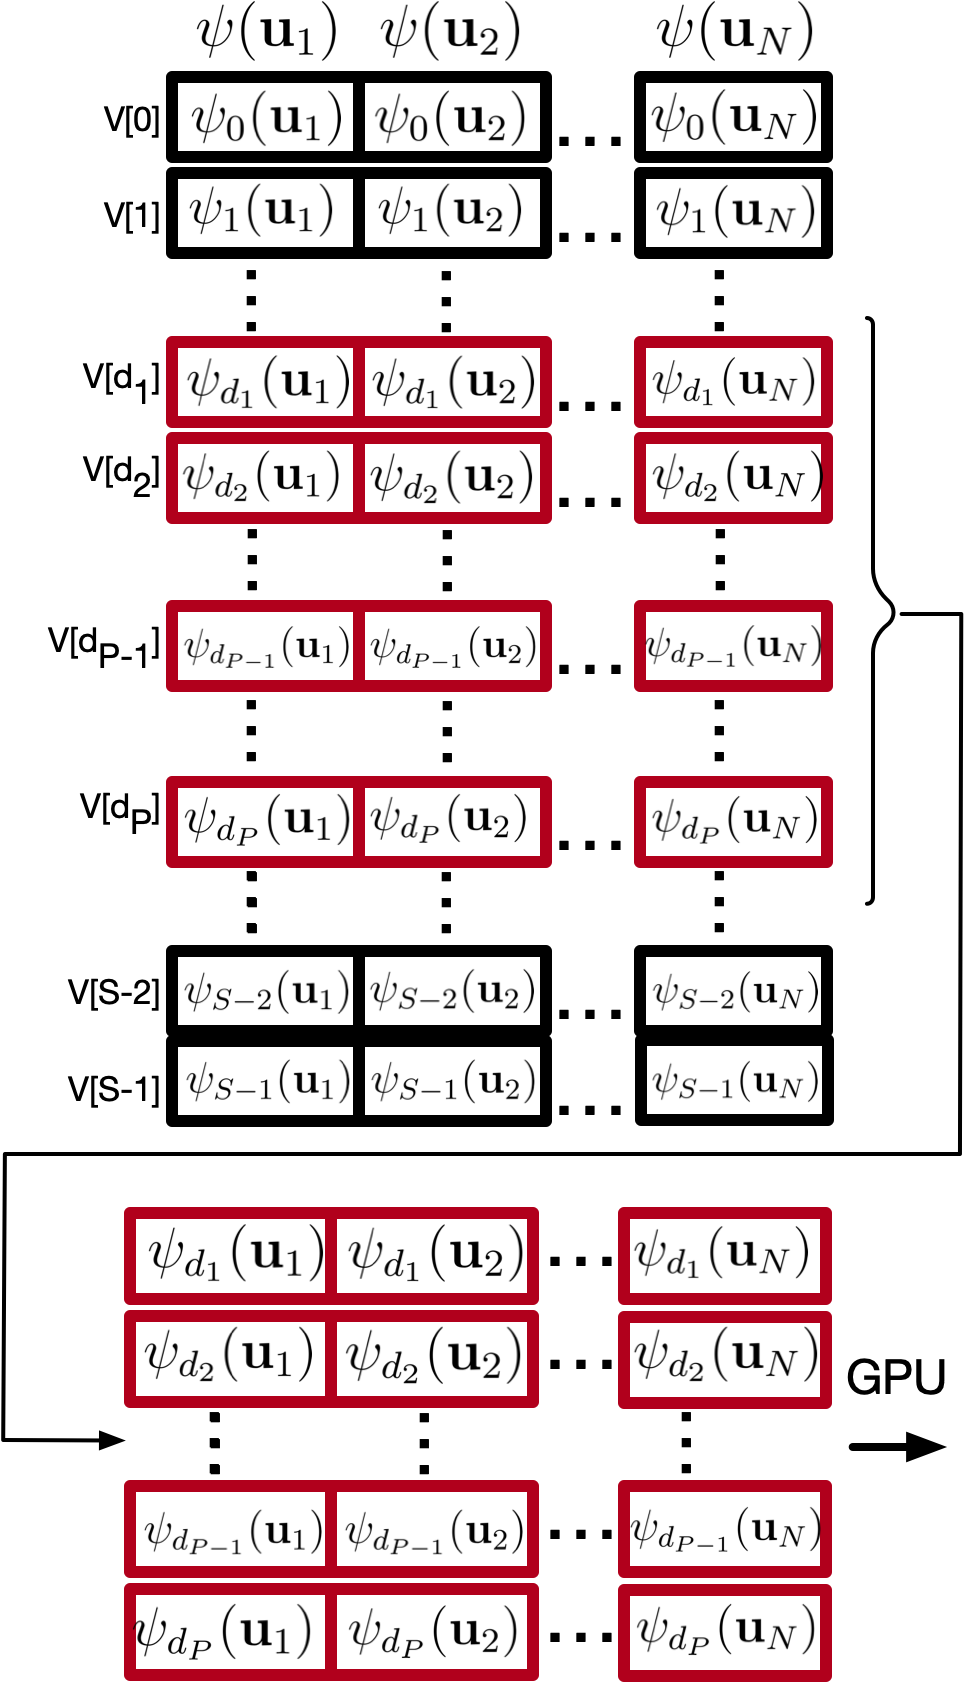
\includegraphics[width=0.89\linewidth, angle=0]{figs/rendering_scheme/organizacao2GPU_red1.png}
    \caption{Rendering scheme applied to a DWI visualization scheme. For each one of the $S$ DWI's samples, its respective ODF is pre-computed in $N$ samples. The $M$ red-contoured data consists of ODFs that are requested to be drawn. They setup $\bm{\Psi}$ and are sent to the GPU. The ODF set to be rendered can refer to a slice or a set of on-screen detected voxels \cite{voltoline2021}.}
    \label{fig::vmtk_precomputed2GPU}
\end{figure}



On the GPU, the access of ODFs to deform its respective sphere point is done by accessing the texture data through its instance and vertex indexes in the vertex shader.

The i-th instance index (Instance\_ID) corresponds to an instanced spherical mesh centered in its respective point $C_{i+1}$, and since ODFs samples of this glyph are stored in the (i+1)-th row of $\bm{\Psi}$, the Instance\_ID access this dimension.

The j-th vertex index (Vertex\_ID), in its turn, indicates the (j+1)-th point of the spherical mesh, which corresponds to the column of its respective ODF value in $\bm{\Psi}$.

Hence, the GPU access is performed by a simple lookup of the texture texel\footnote{In OpenGL, the lookup is done by the command texelFetch($\bm{\Psi}$, ivec2(gl\_InstanceID, gl\_VertexID), 0)[0]} as a function of the Vertex\_ID and Instance\_ID pair. Fig. \ref{fig::GPU2glyph} illustrates the ODF access for each instance and vertex in the GPU.

%(MESMO PARÁGRAFO ACIMA, COM INDICAÇÕES OPENGL)The access in the GPU of ODFs to deform its respective sphere point is done by accessing the texture data through its instance and vertex indexes in the vertex shader. To achieve this, it is necessary that the vertex index (Vertex\_ID) (gl\_VertexID\footnotemark) of the direction of each vertex correspond to the column of its respective ODF value $ \psi (\bm{u}_j) $ in diffusion profile matrix. The access of the rows of the diffusion profile matrix, corresponding to the diffusion profiles in its respective point is accessible by the instance index (gl\_InstanceID\footnotemark [\value{footnote}]). Having the data organized in this established way, the access is done by perfoming a single lookup of the texel in the texture using the Vertex\_ID and Instance\_ID as a pair. In OpenGL, this can be done by the function texelFetch\footnotemark[\value{footnote}] with the row and column access arguments through the pair ( gl\_VertexID, gl\_InstanceID)\footnotemark [\value{footnote}] \footnotetext{All commands refer to OpenGL API and GLSL shading language.}. How to access the GPU of the profile matrix is illustrated in the Fig.\ref{fig::GPU2glyph}.

%\todo[inline]{It is not understandable the caption!!! And it is not clear what is exactly the column and what is the row. It seems that your texture is 3D. columen (vertex\_ID), row (instance\_ID), depth (diffusion profile consisting of a series of values).}

\begin{figure}[htb]
    \centering
    %\rule{6cm}{3cm}
    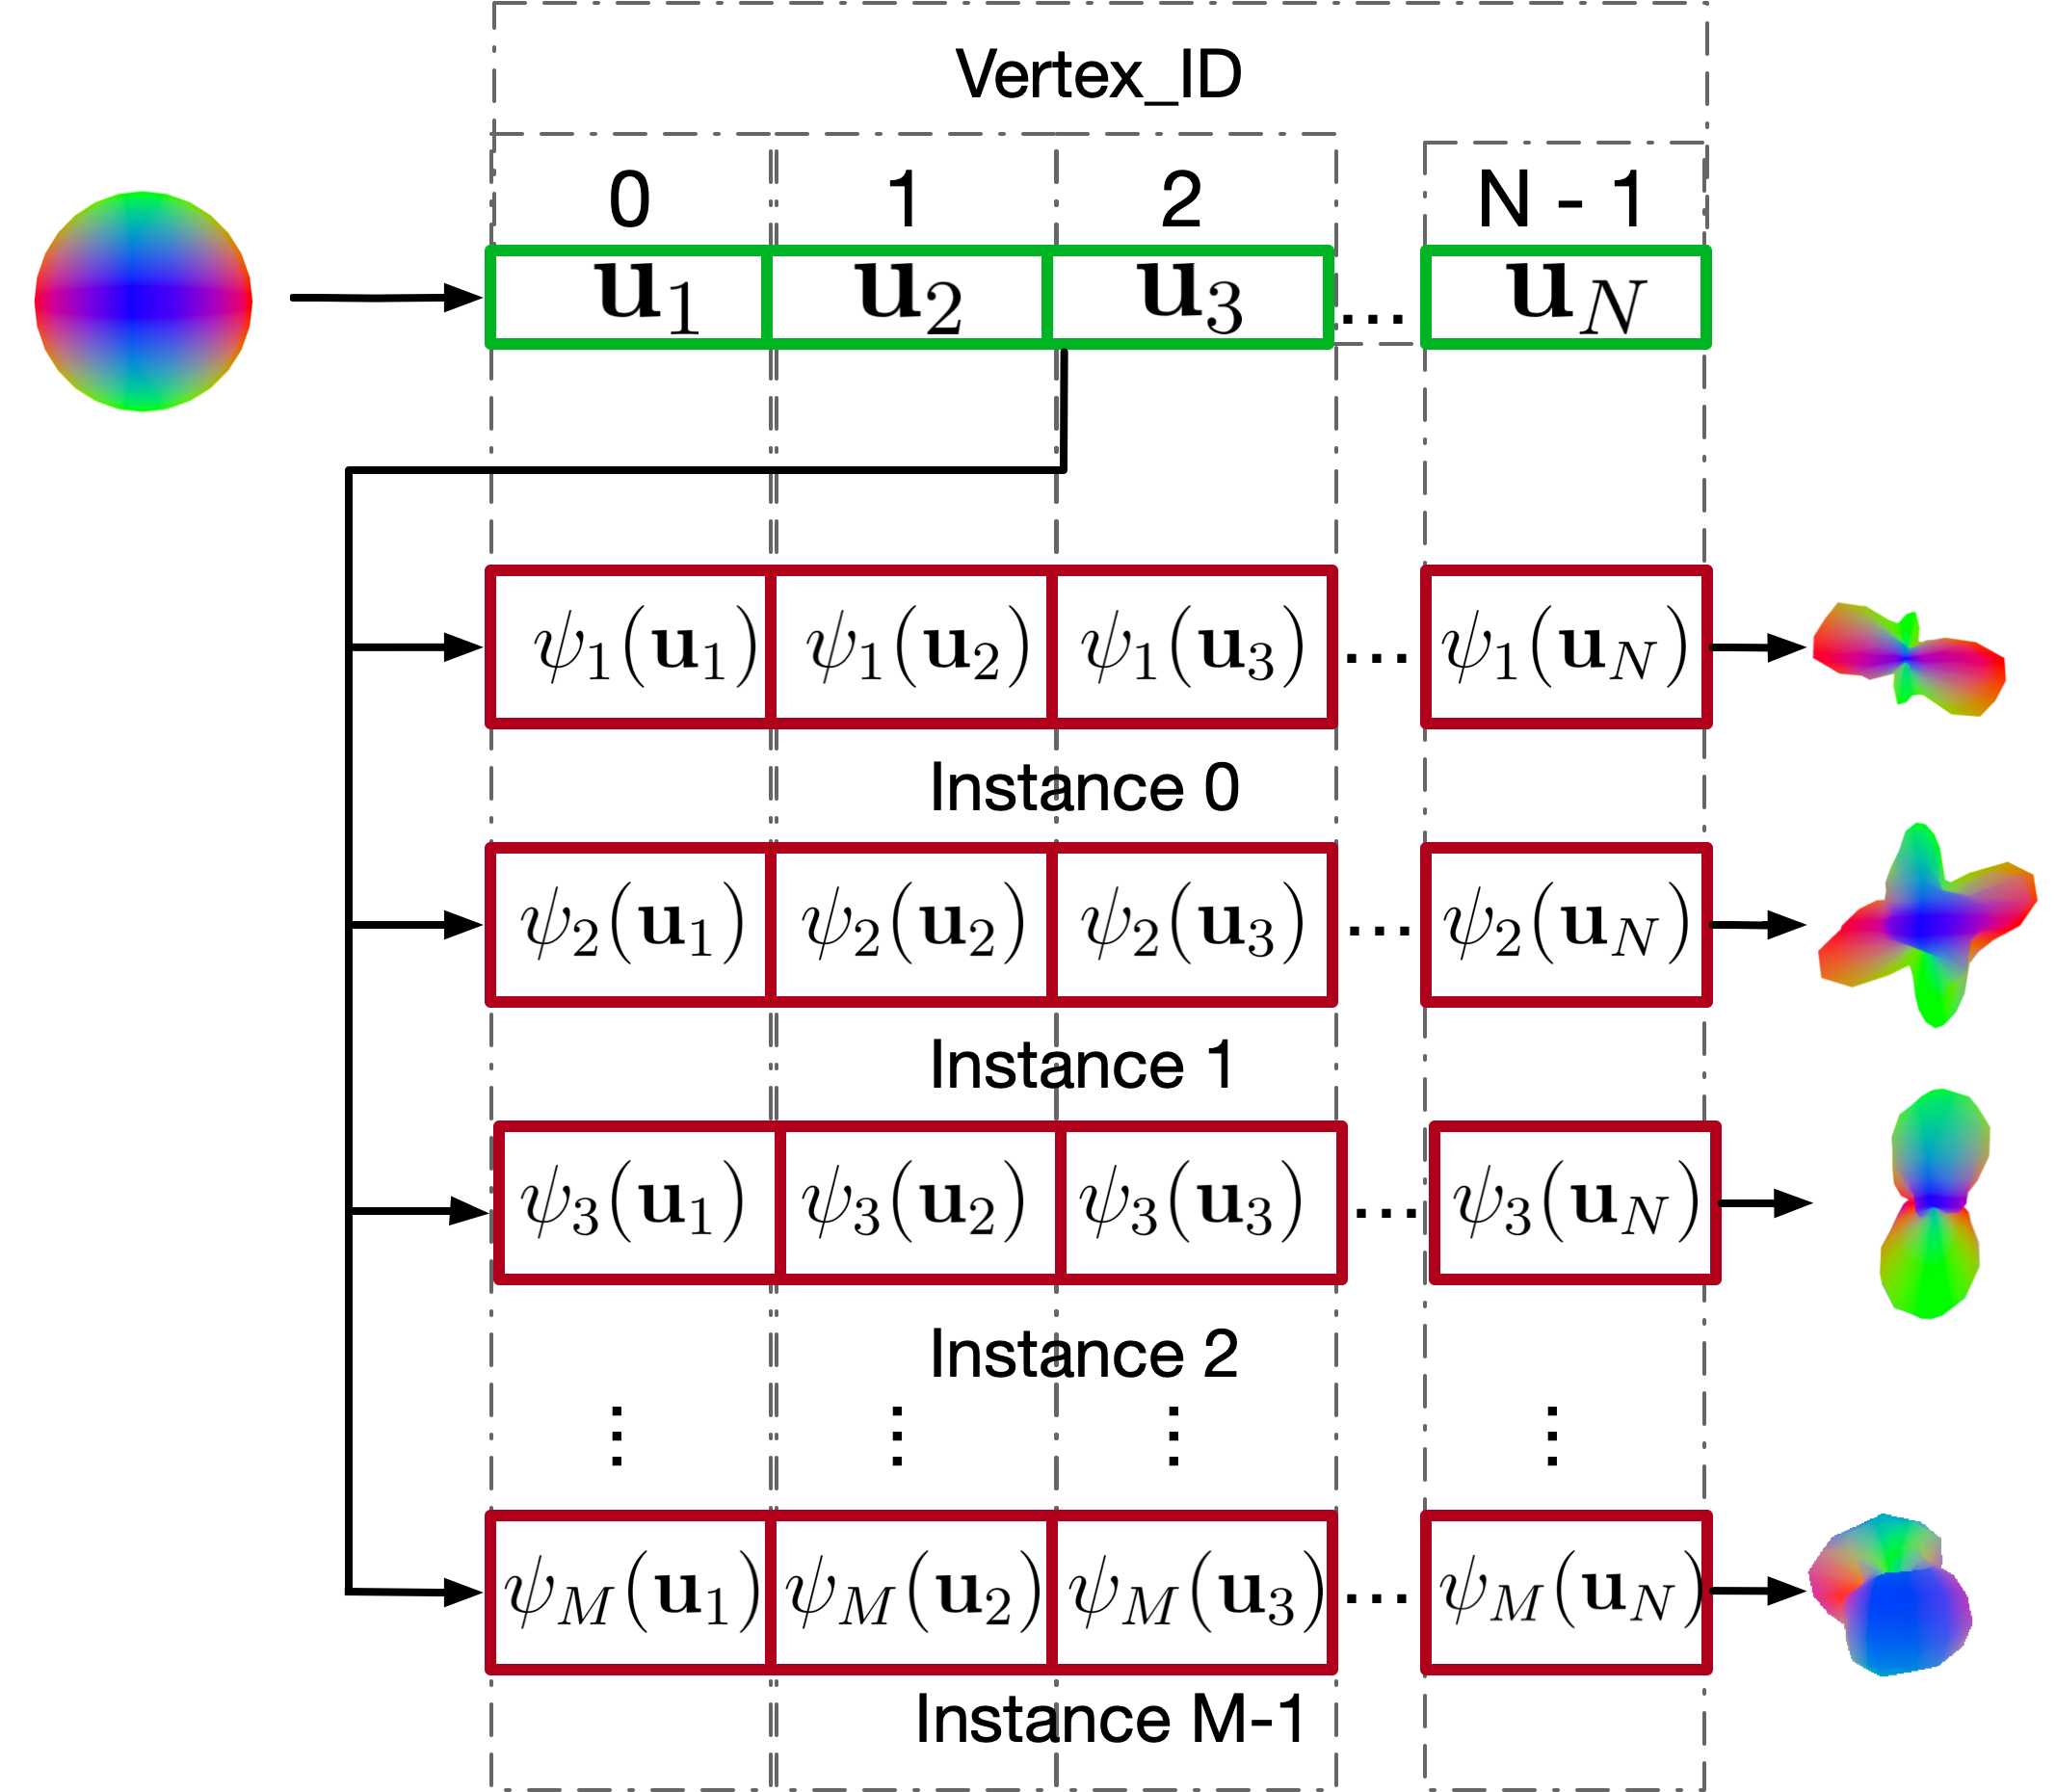
\includegraphics[width=1.0\linewidth, angle=0]{figs/rendering_scheme/GPU2Glyph.png}
    \caption{
    Illustration of $\bm{\Psi}$ (in red) and its lookup procedure in the vertex shader by its Vertex\_ID and instance indexes for $M$ glyphs to be rendered. The data structure of $\Upsilon$ is in green. For an ODF $\psi_i(\bm{u})$, the value recovered for each $\mathbf{u}_j$ scales its respective mesh point $P_j$, deforming it.
    %\textcolor{red}{Illustration of the data organization in the GPU of the profile matrix (red) sent as 2D-Texture. The vertices of the spherical mesh are in green. At each instance, the customization of the glyph occurs through the multiplication of the mesh vertex with its respective value, recovered in the vertex shader through its vertex index for the P glyphs to be rendered}.
    }
    \label{fig::GPU2glyph}
\end{figure}

%\section{Scheme Overview}
%\label{sec::scheme_overview}
%\subsection{Precomputation}
%\begin{enumerate}
%    \item Compute spherical mesh and its index buffer and send to GPU.
%\end{enumerate}
%\subsection{CPU}
%\begin{enumerate}
%    \item Compute matrix $\bm{\Psi}$ and send to GPU as a texture.
%\end{enumerate}
%\subsection{GPU}
%\subsubsection{Vertex Shader}
%\begin{enumerate}
%    \item Lookup the coefficient that customize the glyphs and multiply by the spherical vertex;
%    \item perform translation of the glyph;
%    \item do scaling and camera related transformations;
%    \item compute color as a function of the spherical mesh vertex accordingly to equation %\ref{eq::glyph_color} and send to fragment shader.
%\end{enumerate}
%\subsubsection{Fragment Shader}
%\begin{enumerate}
%    \item Set the output color as the rasterized color defined in the vertex shader.
%\end{enumerate}

\subsubsection{Optimization on symmetrical ODFs}
\label{sssec::optimization}

This subsection shows an adaption of the data structure described in the subsection \ref{ssec::datastruct} to symmetrical ODFs and a strategy to decrease its related CPU-GPU data traffic by half.

An ODF is symmetrical if $\psi(\bm{u}) = \psi(-\bm{u})$ for all $\bm{u}$ in the unit sphere. This symmetry applies to the diffusion behavior, which makes this section entirely applicable for rendering HARDI ODFs.%This property is present on all imaging methods for diffusion.

Firstly, we suggest the use of a symmetrical spherical mesh. That means, if a point $P \in \Pi \implies -P \in \Pi$ as well. %As an example, a mesh generated by any order of a tessellated icosahedron fits this criterion.

Secondly, we recommend that the chosen symmetrical spherical mesh's data structure is organized so that a point $P$ in an even index is followed by $-P$. This spherical mesh is sent to the GPU in the same structure as stated in the subsection \ref{ssec::precomputation}.

%\textcolor{red}{Firstly, we suggest the use of a symmetrical spherical mesh, which can be, for example, any order of a sphere \todo{How? It must be explained!}generated by a tessellated icosahedron. We suggest as well that the vector containing its vertices is organized in such a way that the vector in the (2k)-th index is symmetrical to the (2k+1)-th.}

Following these recommendations, the data structure of points in the sphere $[P_1, P_2, P_3, P_4, \dots, P_{N-1}, P_N]$ becomes $[P_1, -P_1, P_3, -P_3, \dots, P_{N-1}, -P_{N-1}]$, their associated $\Upsilon$ turns to $[\bm{u}_1, -\bm{u}_1, \bm{u}_3, -\bm{u}_3, \dots, \bm{u}_{N-1}, -\bm{u}_{N-1}]$ and $\bm{\Psi}$ becomes:

\begin{equation*}
\bm{\Psi} = 
\begingroup % keep the change local
\setlength\arraycolsep{2pt}
\begin{bmatrix} 
    \psi_1(\bm{u}_1) & \psi_1(-\bm{u}_1) & \cdots \psi_1(\bm{u}_{N-1}) & \psi_1(-\bm{u}_{N-1})  \\
     \psi_2(\bm{u}_1)& \psi_2(-\bm{u}_1) & \cdots \psi_2(\bm{u}_{N-1}) & \psi_2(-\bm{u}_{N-1}) \\

    \vdots & \vdots & \vdots & \vdots  \\
     \psi_M(\bm{u}_1)&\psi_M(-\bm{u}_1) & \cdots \psi_M(\bm{u}_{N-1}) & \psi_M(-\bm{u}_{N-1})
\end{bmatrix}
\endgroup
\end{equation*}

where each of the (2k+1)-th column is the same as the (2k+2)-th ($0 \leq k < \frac{N}{2}$).

Hence, we define a matrix $\bm{\Psi^h}_{Px\frac{M}{2}}$ such that $\bm{\psi^h}_{ij} = \bm{\psi}_{i(2j-1)}$, which is described in the expression below:

%\todo{Very confusing!}We \textcolor{blue}{re}define \textcolor{blue}{Eq. \ref{eq::Psi}}, \sout{a matrix $\bm{\Psi^h}_{Px\frac{N}{2}}$ where} \textcolor{blue}{such that} $\bm{\psi^h}_{ij} = \bm{\psi}_{i(2j-1)}$. \sout{that is sent to GPU on every drawing request. Its form is stated below:}\textcolor{blue}{It assumes the form}

\begin{equation*}
\label{eq::Psi_changed}
\bm{\Psi^h} = 
\begingroup % keep the change local
\setlength\arraycolsep{2pt}
\begin{bmatrix} 
    \psi_1(\bm{u}_1) & \psi_1(\bm{u}_3) & \cdots \psi_1(\bm{u}_{N-3}) & \psi_1(\bm{u}_{N-1})  \\
    
     \psi_2(\bm{u}_1)& \psi_2(\bm{u}_3) & \cdots \psi_2(\bm{u}_{N-3}) & \psi_2(\bm{u}_{N-1}) \\

    \vdots & \vdots & \vdots & \vdots  \\
    
     \psi_M(\bm{u}_1)&\psi_M(\bm{u}_3) & \cdots \psi_M(\bm{u}_{N-3}) & \psi_M(\bm{u}_{N-1})
    
\end{bmatrix}
\endgroup
\end{equation*}

$\bm{\Psi^h}$ is sent to the GPU in the drawing requests in the same way as $\bm{\Psi}$ described in the subsection \ref{ssec::datastruct} and the difference lies in the lookup process. On the GPU, the vertices corresponding to the 2k-th and (2k+1)-th Vertex\_ID in the spherical mesh of the same instance have the same value to lookup\footnote{In OpenGL, the lookup is done by the command texelFetch($\bm{\Psi^h}$, ivec2(gl\_InstanceID, gl\_VertexID/2), 0)[0]}, corresponding to the k-th column, which can be accessed accordingly in the vertex shader.

%\sout{In}\textcolor{blue}{On} the GPU, the  in $\bm{\Psi}^h$, which corresponds to the K-th index of the matrix, which can be accessed accordingly in the vertex shader.


\subsection{CPU and GPU Algorithms for Rendering Overview}
\label{ssec::rendering}
\subsubsection{CPU}
\begin{enumerate}
    \item Update translation attributes buffer with the $M$ elements to be rendered;
    \item Setup $\bm{\Psi}$ or $\bm{\Psi^h}$ and update its respective 2D texture with the samples to be drawn.
\end{enumerate}

\subsubsection{GPU}
Vertex Shader:
\begin{enumerate}
    \item Lookup the coefficient that customizes the glyphs' vertex; 
    \item perform the scaling on the spherical vertex;
    \item perform the translation of the vertex;
    \item apply view-projection transformation;
    \item compute color as a function of the spherical mesh vertex accordingly to Eq. \ref{eq::glyph_color} and send to the fragment shader.
\end{enumerate}

Fragment Shader:
\begin{enumerate}
    \item Set the output color as the rasterized color set in the vertex shader.
\end{enumerate}


%\section{Optimization}

%\todo[inline]{Is it not better to put together with other part of description?}



\section{Dynamic resolution adjustment}

In this section, we show a strategy to organize ODF samples, so the amount of triangles of the spherical mesh is adaptive and a function of the number of glyphs being rendered.

Voltoline and Wu \cite{voltoline2021} addressed the importance of an adaptive mesh in order to keep the rendering speed and image quality compromise and proposed a computation of the mesh, where the amount of triangles is a function of the size of the glyphs to be rendered in the scene. In their work, they propose an expression that establishes a relation between the mesh's amount of triangles $\tau$ and the maximum amount of pixels containing a single voxel  in a multimodal visualization environment for MRI and superquadrics glyphs ($\max_p$), which is given by:

\begin{equation}
    \tau(max_p) = \lfloor 2(3 + 2\sqrt[4]{max_p})^2 \rfloor
\end{equation}
%They formalize an analytical expression that set the amount of triangles of the superquadrics as a function of the maximum amount of pixels used to render a single raycasted volume's voxel, as shown in Eq. \ref{eq::pixel_res}. Thus, the resolution of the superquadric is adaptative to its respective size, the bigger it is, more details it has.
%!!COLOCAR A EQUAÇÃO DO RAPHAEL.
%\begin{equation}
%    \label{eq::pixel_res}
%\end{equation}

%The equation compensates an advantage of the raycasting approaches over a non-dynamically set mesh's resolution, which is the amount of GPU's computational workload is proportional to the object's size.

%As we proposed an rendering based in ODF samples stored in CPU, we describe a procedure to alternate the instanced spherical mesh on runtime. The ODF samples its vertices are a subset of the vertices of the highest resolution mesh used to sample the ODFs.

!!(MODIFICAR ISSO) The situation where each mesh is adequate is up to the user, and it can be as a function of the glyphs' size \cite{voltoline2021} and/or the amount of them rendered. Thus, we suggest a data structure of the spherical mesh and ODF samples in such a way that when alternating from one resolution to another, the change lies only in the active index buffer in the mesh and the amount of per-glyph ODF samples in CPU-GPU data traffic.

Let $\Pi = \{P_1, P_2, ..., P_{N}\}$ be the vertices of the highest resolution spherical mesh, associated with its index buffer set $I$ and has the ODF samples projected onto it. Let $\Pi_{1}$, $\Pi_{2}$, ..., $\Pi_{t}$ be a set of vertices that define a spherical mesh such that:

\begin{equation}
\label{eq::subset_condition1}
    \Pi_{1} \subset \Pi_{2} \subset \Pi_{3} \subset ... \subset \Pi_{t} \subset \Pi;
\end{equation}
and
\begin{align}
 \label{eq::subset_condition2}
    &\Pi_{1} = \{P_1, P_2,... P_{V_1}\}; \nonumber\\
   % &\Pi_{2} = \{P_1, P_2,... P_{V_1}, P_{V_1+1}, ..., P_{V_2}\} = \Pi_1 \cup \{ P_{V_1+1}..., P_{V_2}\} \nonumber\\
    &\Pi_{2} = \Pi_1 \cup \{ P_{V_1+1}..., P_{V_2}\} \nonumber\\
    &\Pi_{3} = \Pi_2 \cup \{ P_{V_2+1}..., P_{V_3}\} \nonumber\\
    &... \\
    &\Pi_{t} = \Pi_{t-1} \cup \{ P_{V_{t-1}+1}..., P_{V_t}\} \nonumber\\
    &\Pi = \Pi_{t} \cup \{ P_{V_t+1}..., P_{V_N}\}; \nonumber
\end{align}


where $t$ is the amount of subsets of the spherical mesh vertices $\Pi$. The amount of vertices on each mesh follows the property $V_n > V_t > V_{t-1} > ... > V_2 > V_1$. The sets $\Pi_{1}, \Pi_{2}, \Pi_{3}, ..., \Pi_{t}$ have their respective index buffer $I_{1}, I_{2}, I_{3}, ..., I_{t}$ associated to form the triangles. $\Pi_k$ and $I_k$ ($k \leq t$) define the k-th subset of the highest resolution spherical mesh.

In order to provide the possibility of resolution adjustment on the glyphs mesh, we suggest an additional task at the initialization of the rendering scheme. In addition to uploading the mesh's vertices set of the highest resolution $\Pi$ as a data structure $[P_1, P_2, ..., P_N]$ in GPU, alongside its respective index buffer as pointed in the subsection \ref{ssec::precomputation}, we suggest that the $t$ index buffers that form the triangles using the points of $\Pi$'s subsets to be uploaded in the graphics unit.

%The set $\Pi$ is upload on GPU at the initialization as a data structure $[P_1, P_2, ..., P_N]$, as well as all of the index buffers for all meshes derived. The ODF data per glyph is $[\psi_1(\bm{u}_1), \psi_1(\bm{u}_2), \dots, \psi_1(\bm{u}_{N})]$.

One must be attentive to two procedures to select the chosen k-th subset of the highest resolution mesh. The first consists of the activation of the spherical mesh $(\Pi_k, I_k)$ by activating its index buffer $I_k$. The second consists of setting the number of columns $V_k$ that build the ODF matrix sent to GPU, which consists of the $V_k$ first ODF samples, which must be coherent to the vertices of $\Pi_k$. This procedure reduces the ODF matrix size by a factor of $1-V_k/V_n$.






%!!Falar de forma generica por aqui?

\subsection{Example of a two-powered set of tessellated icosahedron meshes}

In this section, we show an application on how to alternate meshes of spherical meshes on ODF's sampled over a two-powered order icosahedron's tessellation.

The sphere obtained by the tessellation of the icosahedron is a set of spherical meshes often used by the HARDI community. Tuch \cite{TuchQBall2004} and Yeh et al., \cite{yeh2010} in their proposed diffusion imaging methods for HARDI works, use this mesh category in their experiments to show the reconstruction of their respective ODFs. Descoteaux et al. \cite{descoteaux2007} use this category of mesh to project an ODF represented by base functions to compute its underlying fiber configuration. Additionally, this mesh is symmetrical, which makes the optimization described in the subsection \ref{sssec::optimization} applicable.

The sphere mesh obtained by two-powered tessellation presents the following property:  for $k < n$, the vertices of the $2^{k}$ order tessellated icosahedron is a subset of $2^{n}$. The tessellation of order $2^k$ consists in a subdivision of each triangle of the $2^{k-1}$ tessellation in four. These four triangles vertices' are formed by six points: three comes from the base triangle from $2^{k-1}$-th order, and the other three are derived from these points as they are each pair's projection of the median points onto the sphere as illustrated in Fig. \ref{fig::subdivision_icosahedron}. Table \ref{tab::icosahedron_set} shows the amount of vertices and triangles of each tessellation order.

\begin{figure}[ht]
    \centering
    %\rule{6cm}{3cm}
    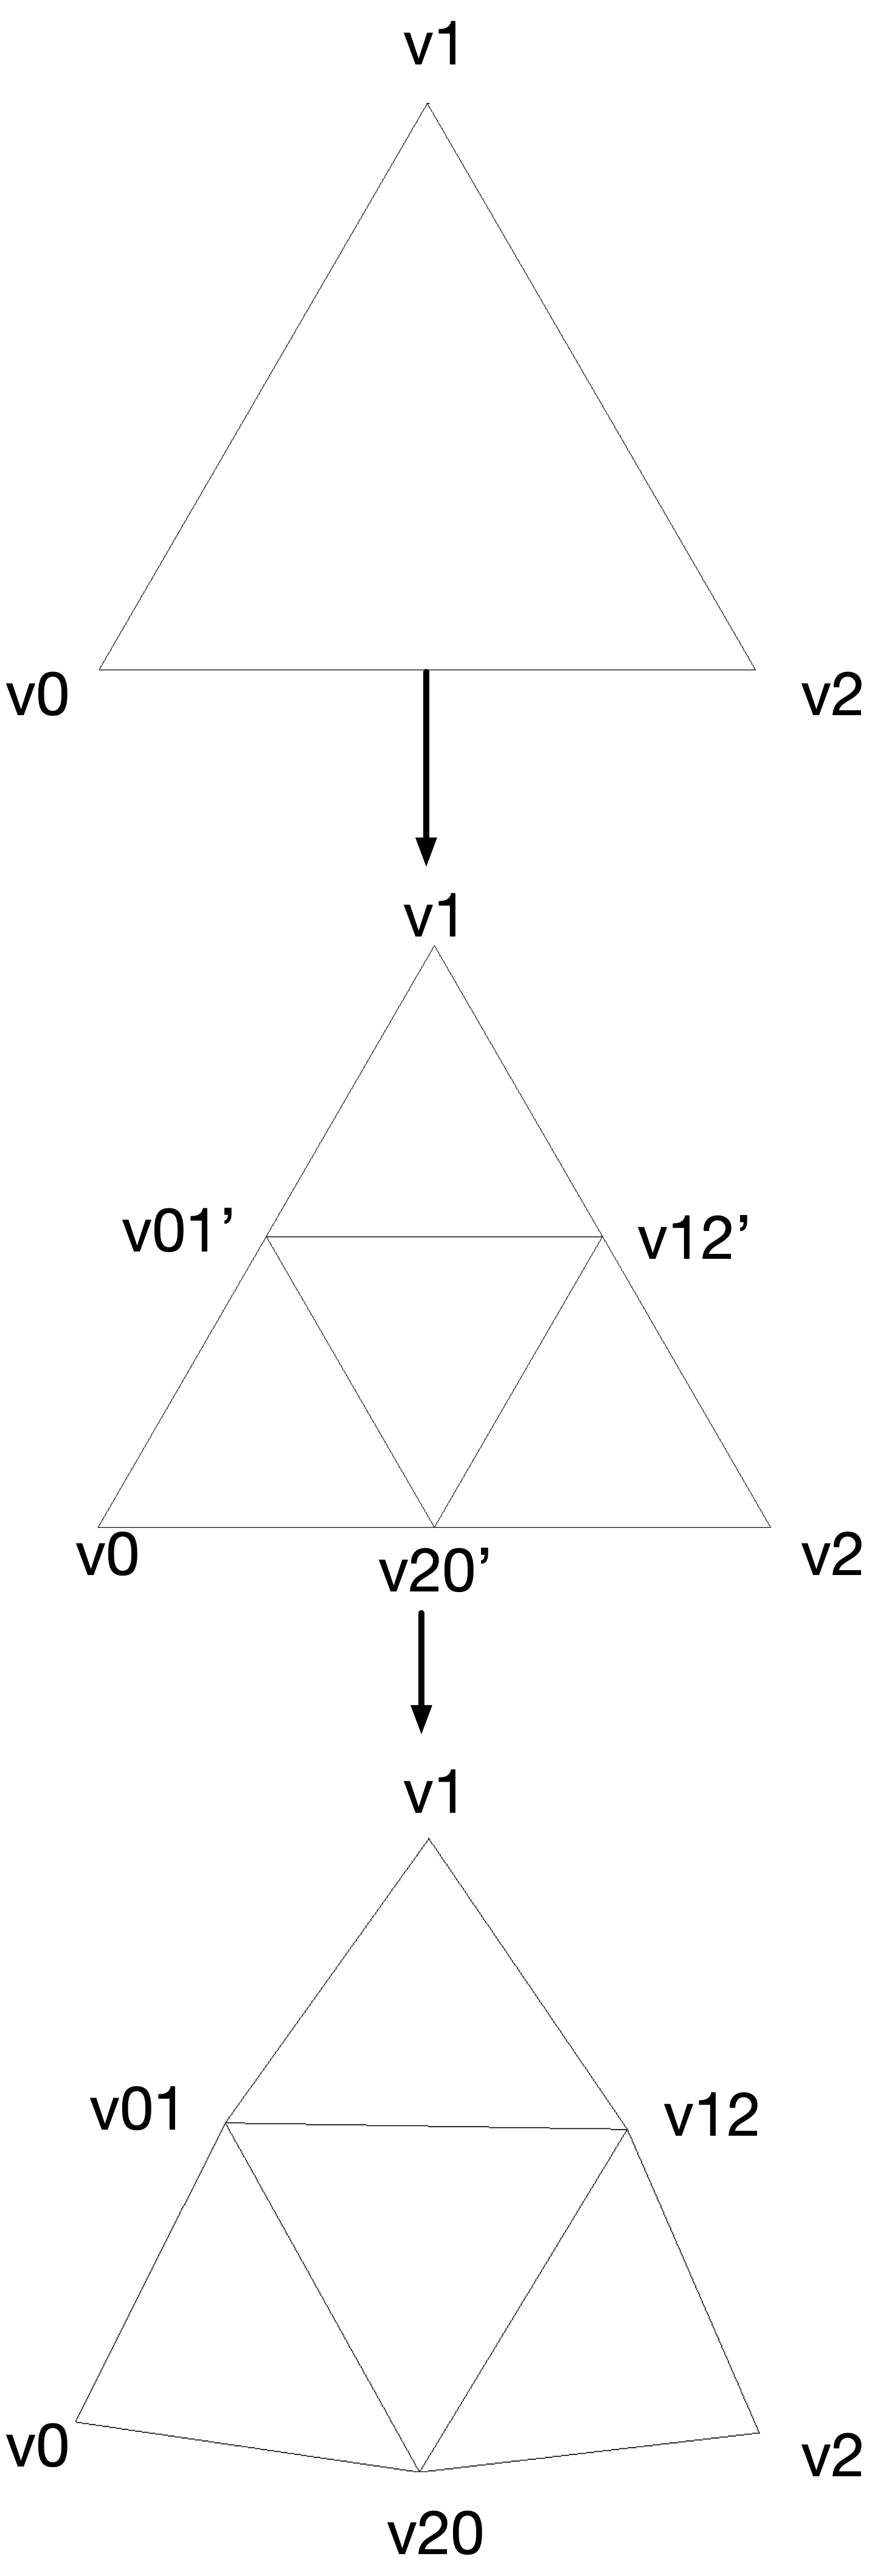
\includegraphics[width=.50\linewidth, angle=0]{figs/icosahedron_example/ico_subdivision_V.png}
    \caption{Triangle subdivision to form a $2^k$-th order of tessellation of the icosahedron from a $2^{k-1}$-th order. The triangle formed by v0, v1, and v2 is subdivided into four triangles, where the median points v01', v12'and v20' are computed and their projections on the unit sphere v01, v12, and v20 are added into the vertices set.
    }
    \label{fig::subdivision_icosahedron}
\end{figure}



Thus, assigning $\Pi$ to be the vertices set of the $2^k$-th order of tessellation of the icosahedron and $\Pi_1$, $\Pi_2$, ..., $\Pi_{k-1}$ to be the $2^{1}$-th, $2^{2}$-th, ..., $2^{k-1}$-th order, respectively, we obtain a set of meshes that satisfy the properties described in the expressions \ref{eq::subset_condition1} and \ref{eq::subset_condition2}. In practice, we recommend $k$ to be equal to 3 or 4, which corresponds to 642 and 2562 samples on the sphere. Values of k above that may occur in a prohibitive amount of memory for ODF samples in a DWI.

%In this section, we are going to consider $\Pi$ as the points of the spherical mesh generated by the $16^{th}$ tessellation order of the icosahedron, which gives $V_N = 2562$ points. Thus, $\Pi_1$, $\Pi_2$ and $\Pi_3$ are the vertices set of the $2^{nd}$, $4^{th}$ and $8^{th}$ order of the tessellated icosahedron, respectively. They 

\begin{table}[]
\centering
\begin{tabular}{|c|c|c|c|}
\hline
\textbf{Order} & \textbf{\#Vertices} & \textbf{\#Triangles} \\ \hline
1              & 12                 & 30                  \\ \hline
2              & 42                 & 120                 \\ \hline
4              & 162                & 480                 \\ \hline
8              & 642                & 1920                \\ \hline
16             & 2562               & 7680                \\ \hline
$2^k$          & $10(2^k+1)(2^k-1)+12$ & $30.4^k$           \\ \hline
\end{tabular}
\caption{Amount of vertices and triangles of 2-powered order tessellation of the icosahedron. For $k<n$, the vertices on the tessellation $2^k$ is a subset of $2^n$.}
\label{tab::icosahedron_set}
\end{table}

%Let the set $\Pi_{16} = \{P_1, P_2, ..., P_{2562}\}$ to be correspondent to the $16^{th}$ tessellated icosahedron. Then, we suggest that the data is organized in such a way that its respective subsets $\Pi_{2^k}$, $(k<4)$ is $\{P_1, P_2, ..., P_{V_{2^k}}\}$.

%It means that the first 12 vertices of $\Pi_{16}$ corresponds to the icosahedron's vertices, the first 42 vertices correspond to the $2^{nd}$ order tessellation, the 162 first vertices corresponds to the vertices of the $4^{th}$ tesselation, and the 642 first elements are the points of the $8^{th}$.

%It means $\Pi_1 = \{P_1, P_2, ..., P_{12}\}$ is the vertices set of the icosahedron; $\Pi_2 = \{P_1, P_2, ..., P_{42}\}$, the vertices of the $2^{nd}$ order of the tessellated icosahedron; $\Pi_4 = \{P_1, P_2, ..., P_{162}\}$, the vertices of the $4^{th}$ order and $\Pi_8 = \{P_1, P_2, ..., P_{642}\}$, the $8^{th}$ tessellation order.

%Organizing the vertices lists eases the ODF-related CPU-GPU data traffic. When the glyph is derivated for a $2^k$ order of the tesselation of the icosahedron, the data traffic consists of the first $V_{2^k}$ ODF samples in CPU.

%We suggest that the vertices set of the $16^{th}$ order of the tessellation of the icosahedron is downloaded in the GPU, as well as the index buffers of each order of the icosahedron that are a subset as well.

%Whenever the resolution of the mesh changes, the additional processes that occurs consists on changing the active index buffer to the requested tessellation and the modification on the amount of elements that set $\bm{\Psi}$ or $\bm{\Psi^h}$.

\section{Results}
\label{sec::results}

\subsection{Visual aspects}

Fig. \ref{fig::ex_glyph} shows glyphs for different meshes in detail. One can see that a spherical mesh defined by an $8^{th}$ (Fig. \ref{fig::ex_glyph8}) tessellation order of the icosahedron is fine enough that it does not have much visual difference compared to the $16^{th}$ order (Fig. \ref{fig::ex_glyph16}).

Fig. \ref{fig::ex_glyph_DWI_visualization} shows an application of the proposed scheme integrated into a DWI visualization system. At that size, one can not infer the shape of the glyphs, and the color is more dominant on the information given. In this scenario, there is an opportunity to decrease glyph resolution to decrease GPU memory usage.

\begin{figure}[ht]
\centering
\captionsetup[subfloat]{farskip=0pt,nearskip=0pt}
    \subfloat[4-th order (162 vertices and 320 triangles per glyph). ]{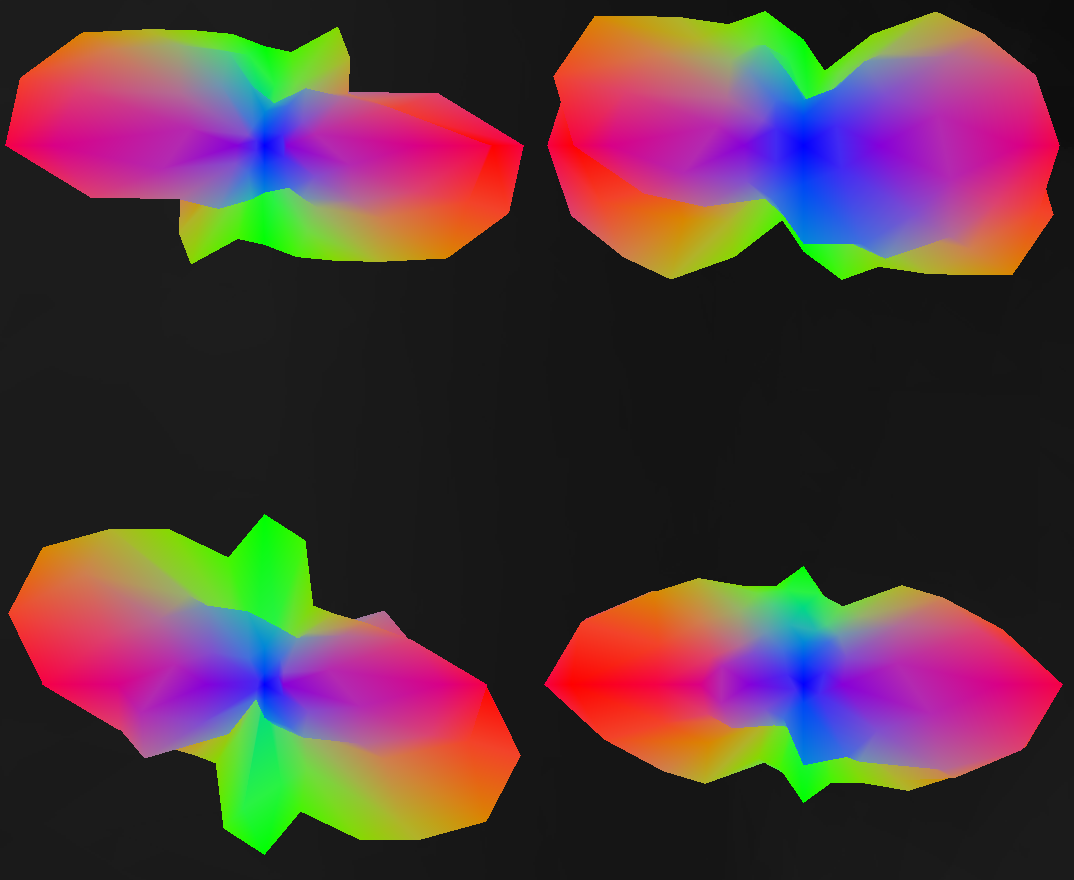
\includegraphics[width=.75\linewidth, angle=0]{figs/Results/Glyphs_4.png}
    \label{fig::ex_glyph4}
    }
    \\
    \subfloat[8-th order (642 vertices and 1280 triangles per glyph). ]{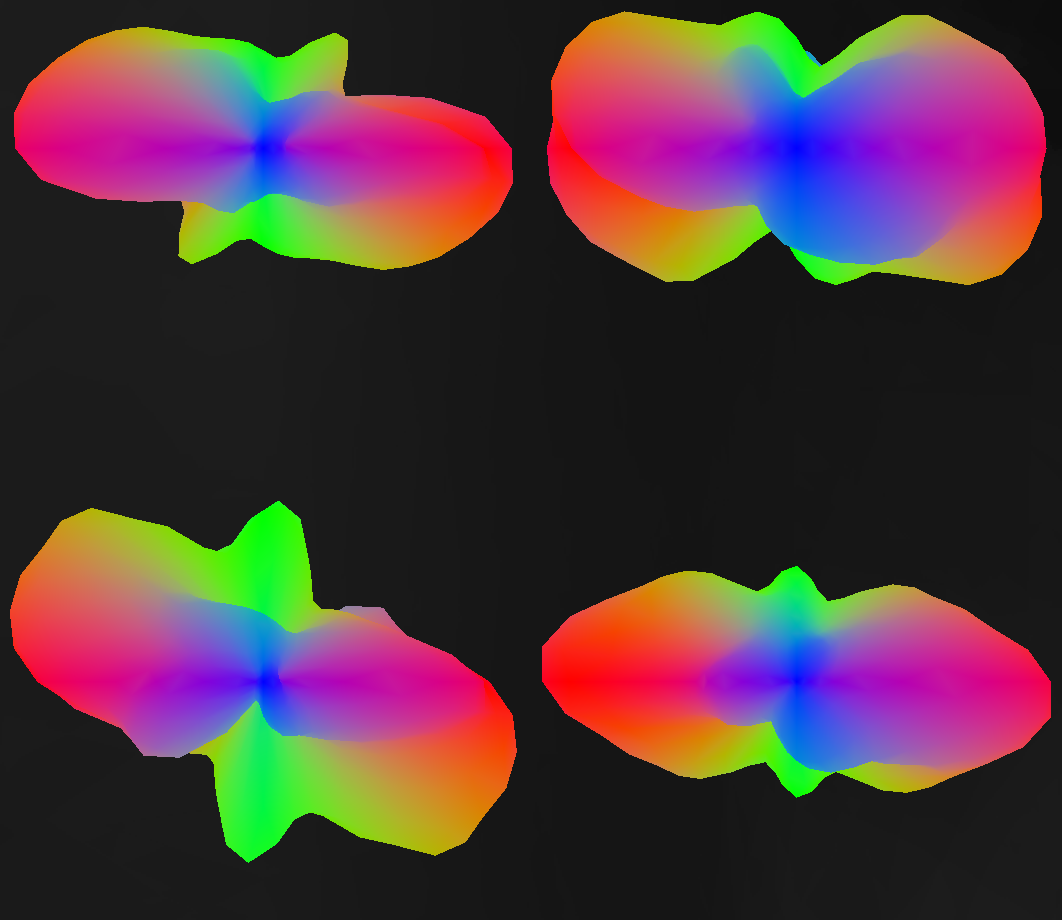
\includegraphics[width=.70\linewidth, angle=0]{figs/Results/glyphs_8.png}
    \label{fig::ex_glyph8}
    }
    \\
    \subfloat[16th order (2562 vertices and 5120 triangles per glyph).    ]{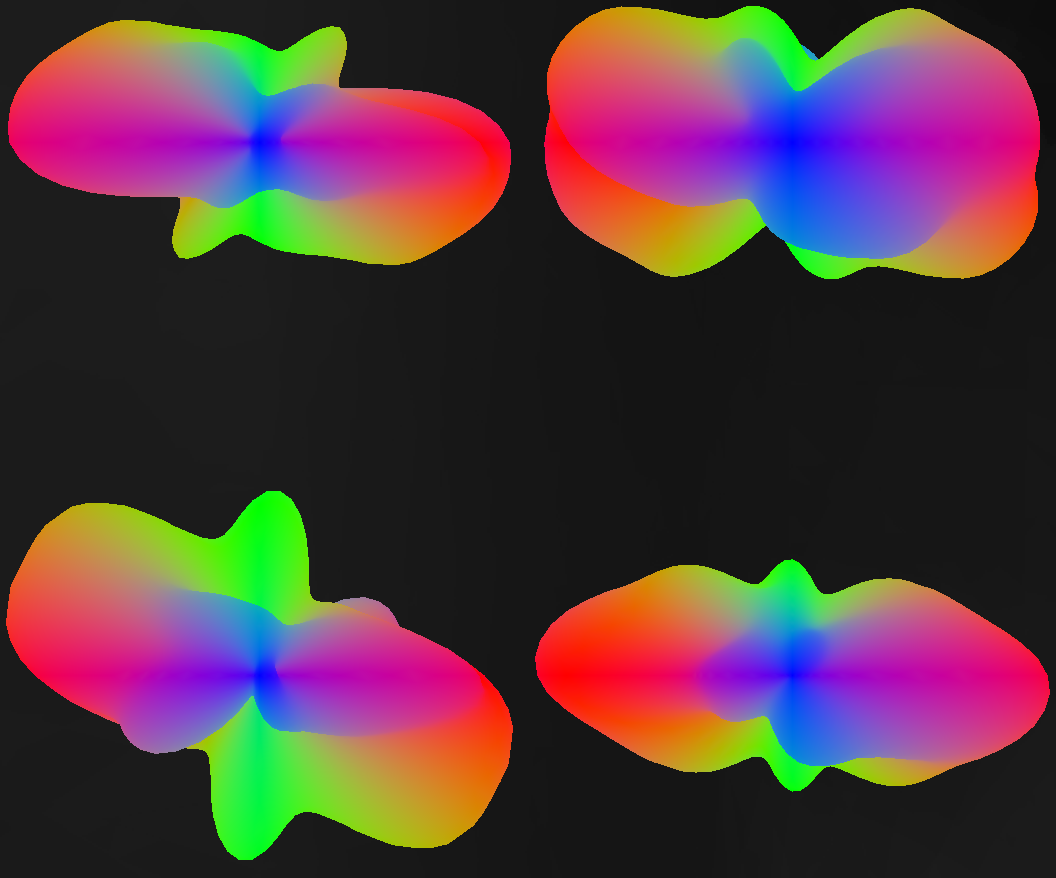
\includegraphics[width=.70\linewidth, angle=0]{figs/Results/glyphs_16.png}
    \label{fig::ex_glyph16}
    }
     \caption{Polygon based HARDI glyphs visualization for different orders of tessellation of an icosahedron. The glyphs refer to the same DWI samples, with 32 gradient directions and b=1000$s/mm^2$. } %!!VER SE ISSO TA CERTO
    \label{fig::ex_glyph}
\end{figure}



%\begin{figure}[ht]
    %\centering
    %\rule{6cm}{3cm}
    %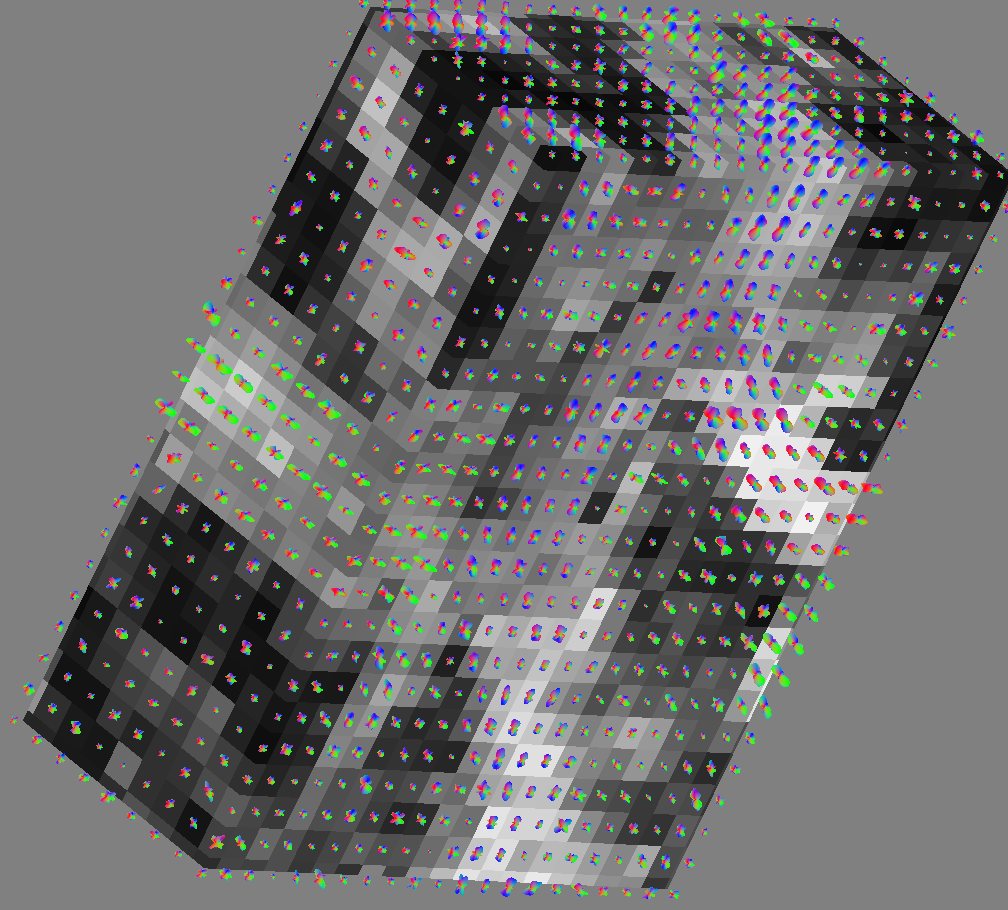
\includegraphics[width=1.00\linewidth, angle=0]{figs/Results/Glyphs_onFAMAP_2.png}
    %\caption{Glyphs integrated into a DW-MRI's fractional anisotropy map. The parallelepiped shows the region where the pyramidal tract (glyphs predominantly blue) crosses the corpus callosum (predominantly red). In the middle of the left face, the predominantly green glyphs corresponds to the region of the superior longitudinal fasciculus. The spherical mesh used corresponds to an 8-th tessellated icosahedron}
    %\label{fig::ex_glyph_FAMAP}
%\end{figure}

\subsection{Performance}

In Fig. \ref{fig::benchmark_full} and \ref{fig::benchmark_half} follow the benchmark of the rendering scheme without and with the optimization for symmetrical ODFs. The data structures setup process is accelerated by using CPU parallelism. The computer used was a Macbook Pro Retina 13' early 2015, with an Intel Core i5 Dual-Core 2.7GHz CPU, 8 GB RAM, and an Intel Iris 6100 GPU with 1536 MB of memory.


\begin{figure}[ht]
\centering
\captionsetup[subfloat]{farskip=0pt,nearskip=0pt}
    \subfloat[General rendering scheme for ODFs benchmark ]{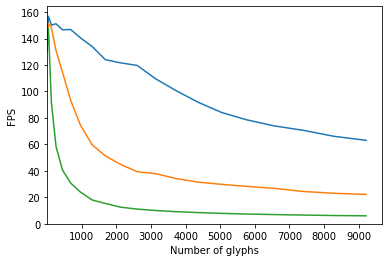
\includegraphics[width=.99\linewidth, angle=0]{figs/Benchmark/benchmark_full.png}
    \label{fig::benchmark_full}
    }
    \\
    \subfloat[Optimized rendering scheme for symmetrical ODFs benchmark ]{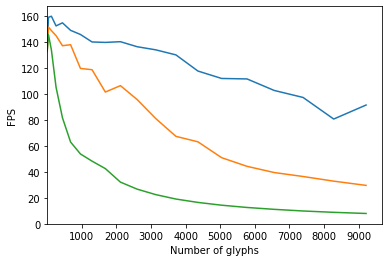
\includegraphics[width=.99\linewidth, angle=0]{figs/Benchmark/benchmark_half.png}
    \label{fig::benchmark_half}
    }
    \\
     \caption{Glyph rendering FPS $\times$ number of glyphs being rendered. The blue, orange and green curves correspond to a spherical mesh  generated by $4^{th}$, $8^{th}$ and $16^{th}$ order tessellation of the icosahedron. Their amount of vertices and triangles are in the table \ref{tab::icosahedron_set}} %!!VER SE ISSO TA CERTO
    \label{fig::benchmark}
\end{figure}

The results indicate that our scheme gives satisfactory results for interactive usage. Using this scheme, it is possible to render thousands of glyphs in interactive rates using a $4^{th}$ order tessellation of the icosahedron and hundreds with $16^{th}$ order, as shown in Fig. \ref{fig::benchmark_half}.

There is a relevant performance difference in the scheme by taking advantage of the ODF's symmetry. For example, in the 642 vertices spherical mesh, without optimization, the graphic hits 60 FPS with less than 2000 glyphs rendered, while taking advantage of the symmetry of ODFs makes it possible to render 4000, obtaining similar performance.




%If the ODFs are stored as coefficients of spherical harmonics, it needs a step of sampling over a spherical mesh.


%Mention comparison with raycasting methods



\subsection{Application}

In this section, we describe the implementation of the rendering scheme in a multimodal visualization environment with DWI functionalities \cite{VMTKNeuro}. Fig. \ref{fig::ex_glyph_DWI_visualization} show the result of the proposed rendering scheme applied to this environment.

\begin{figure}[ht]
    \centering
    %\rule{6cm}{3cm}
    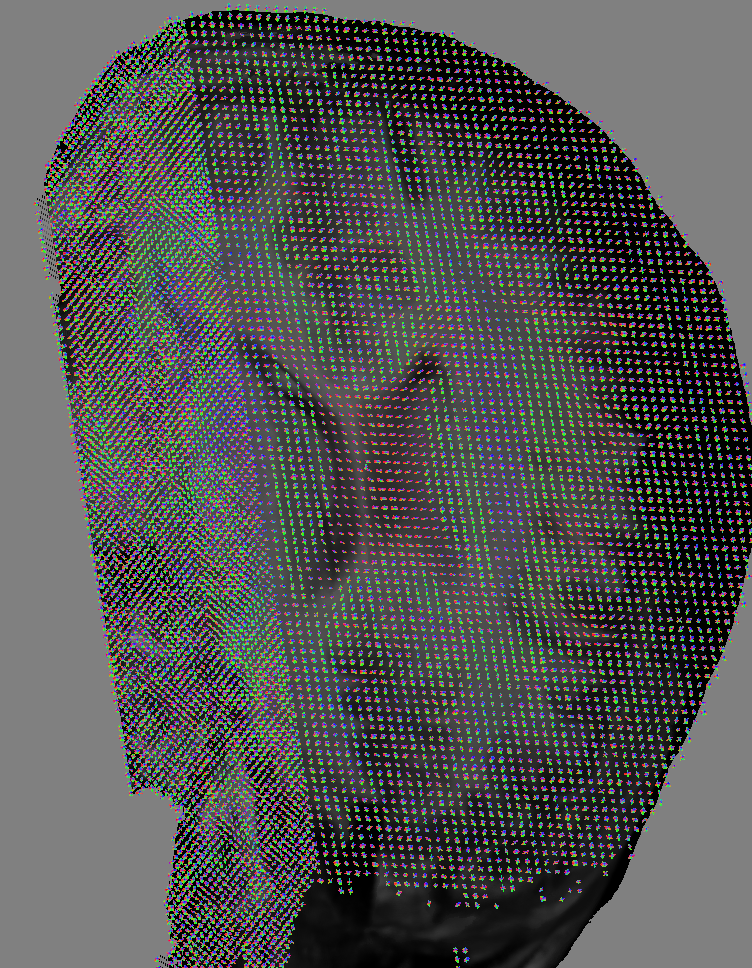
\includegraphics[width=1.00\linewidth, angle=0]{figs/Results/glyphs_integrated_DWI.png}
    \caption{Glyphs integrated into a DWI's visualization scheme. The glyphs are located in a mid axial region of the brain, cut in the left side. The spherical mesh used to generate the glyphs corresponds to an 8-th tessellated icosahedron. The DWI was acquired with 32 gradient directions and $b=1000s/mm^2$.
    }
    \label{fig::ex_glyph_DWI_visualization}
\end{figure}

In this environment, there is a ray casting-based rendering for MRI/DWI volumes and a system for appearing samples detection proposed and described by Voltoline and Wu \cite{voltoline2021}. 

In this environment, a HARDI method is computed and stored through its samples in a hemisphere of a spherical mesh for all samples contained in a DWI, as well as their respective translation coordinates to its center in the volume space.

The visualization system renders the DWI volume, with the option to co-register with its respective anatomical T1 MRI, and the glyphs are rendered at their respective samples position.

To make this possible, the tool that detects the appearing samples on-screen returns their respective indexes of the volume, which serves as the basis for the setup of the translation coordinates buffer and ODF data. The setup is made by copying the pre-computed data into the format discussed in the subsection \ref{ssec::datastruct} and sent to GPU. This process to ODF samples is illustrated in Fig. \ref{fig::vmtk_precomputed2GPU}.




%\todo[inline]{To assess the fiber orientations locally?}

\subsection{Discussion}

One can make a comparison in a scheme where the per-glyph data traffic consists of vertices of triangles. Let us consider a $N$-sized spherical mesh, where each point is a vertex of 6 triangles, which is characteristic of a tessellated icosahedron. The data traffic of our approach per glyph consists of N/2 numbers plus one copy of translate coordinates, and the customization of the glyphs is done per vertex in parallel in the GPU. The information on how to set the triangles is provided once in the initialization process.

The polygon-based approach proposed by Shattuck et al. \cite{shattuck2008} does not discuss the data structures sent to GPU in each drawing request and mentions that they did not use GPU programming; furthermore, instance rendering was not available when the work was proposed. Certainly, the glyph customization is done in CPU, and the data traffic CPU-GPU consisted of a set of vertices extracted from the used spherical mesh with some redundancy so that the graphics API can form the polygons. It means that the amount of vertices data traffic is higher than $N$, corresponding to more than $3N$ numbers for each glyph. Hence, the data traffic of our approach is less than 1/6 for the same spherical mesh.

%In our approach, that amount of data traffic goes to N/2 floats. Other polygon-based approaches, such as using sending vertices of the glyphs associated to an index buffer, makes the data traffic go to 3N floats plus the size of index buffer and, additionally, regarding translation coordinates, one can choose to send this data as an attribute per vertex and increase the data traffic by 3N floats and do on GPU's threads, or the operation can be done on CPU, which is less efficient than sending once per geometry.

%Shattuck et al. \cite{shattuck2008}  do not discuss the data structures sent to GPU in each drawing request and mention that they did not use GPU programming, so 

%the data traffic to setup a glyph is 6 times the same (x,y,z) coordinate of the modulated point, which translate to 18*N floats. If using triangle fan, where the same vertice can define two triangles, that amount goes to 9*N floats



%Albeit we presented means to decrease CPU-GPU data traffic on this polygon-based approach, it is still much higher than the ray casting approaches. In their work, Peeters et al. \cite{peeters2009} mentions a data-traffic of 15 spherical harmonics coefficients per glyph and obtain smoother results than $3^{rd}$ and $4^{th}$ order tessellation of an icosahedron.


%In contrast, these rendering strategies makes possible to increase the resolution of the sphere.

%In comparison with Peeters et al. \cite{peeters2009}, our approach has more data traffic, but the GPU shaders are much simpler an less intensive computationally than the approach suggested in their work.

%Falar da simplicidade é algo relevante?
%In our approach, the GPU shaders are much simpler than the raycasting approach since it only does a lookup on a texture and per-vertex linear transformations, while ray casting approaches bring are more computationally expensive.

%In MRI visualization tools, one may code a HARDI ODFs in two different ways: samples on a sphere and spherical harmonics coefficients. This rendering scheme is straightforward to be used when the data is coded in samples on a sphere, but approach to store HARDI data can be very memory demanding.



\section{Conclusions}
\label{sec::conclusions}

In this work, we presented a rendering scheme to render multiple ODFs at interactive rates. We used a polygons-based approach and suggested procedures to decrease the data traffic CPU-GPU in drawing requests.

We also suggested an optimization procedure to decrease the data computation and CPU-GPU data traffic by half on symmetrical ODFs.

The rendering scheme proved to be fast enough to render hundreds and thousands of objects using meshes that are fine sufficiently to make the surfaces appear smooth, depending on the spherical mesh used.

This scheme can be integrated with other DW-MRI and MRI visualization schemes, and we exemplified the application of it as the integration in our visualization tool for DWI.

To our knowledge, this scheme, alongside the ray casting approaches \cite{peeters2009,almsick2011}, are the ones that give the possibility for fast and interactive HARDI data exploration.

The rendering scheme is not only DWI applicable, but to other areas that use ODFs, represented by its samples.

%It can be a useful tool to render each ODF's glyph on its respective area in the scene.

%\section{Future works}

%For future works, we will do the following investigations
%\begin{itemize}
%\item provide in-depth a performance comparison between the ray casting approach with the approach suggested in this work;
%\item adapt the scheme by changing the data that customize the glyphs from ODF samples to spherical harmonics basis coefficients and compute its samples in GPU;
%\item investigate strategies to change the spherical mesh as a function of the amount and size of glyphs to be rendered in a drawing request, giving the possibility of decreasing its number of vertices in situations where glyphs are small and/or in high number in the scene.
%\end{itemize}







%\section{Page size}
%Permission to make digital or hard copies of all or part of this work for personal or classroom use is granted without fee provided that copies are not made or distributed for profit or commercial advantage and that copies bear this notice and the full citation on the first page. To copy otherwise, or republish, to post on servers or to redistribute to lists, requires prior specific permission and/or a fee. 

%All material on all pages should fit within a rectangle of 16 x 23.7 cm (6.3"x 9.33"), centered on the page horizontally, beginning 2.5 cm (1") from the top of the page and ending with 3,5 cm (1.4") from the bottom.  The right and left margins should be 2.5 cm (1"). The text should be in two 7.6 cm (3") columns with a 0.8 cm (0.3") gutter. 

%\section{Typeset text}
%\subsection*{Normal or Body Text}
%Please use a 10-point Times Roman font, or other Roman font with serifs, as close as possible in appearance to Times Roman in which these guidelines have been set. The goal is to have a 10-point text, as you see here. Please use sans-serif or non-proportional fonts only for special purposes, such as distinguishing source code text. If Times Roman is not available, try the font named Computer Modern Roman. On a Macintosh, use the font named Times.  Right margins should be justified, not ragged.

%\subsection*{Title and Authors}
%The title (Helvetica 18-point bold), authors' names (Helvetica 10-point) and affiliations (Helvetica 10 point) run across the full width of the page -- one column wide. We also recommend e-mail address (Helvetica 10 point). See the top of this page for three addresses. If only one address is needed, center all address text. For two addresses, use two centered tabs, and so on. For more than three authors, you may have to improvise.\footnote{If necessary, you may place some address information in a footnote, or in a named section at the end of your paper, but margins must remain empty.} 

%\subsection*{First Page Copyright Notice}
%Please include 3.8 cm (1.5") text box with the text shown at the bottom of the left column of the first page with the copyright notice.

%\subsection*{Others Pages}
%Others pages start at the top of the page (margin 2.5 cm) and continue in double-column format.  The two columns on the last even page should be as close to equal length as possible. 

%{\bfseries Total length of a paper is max. 8 pages.}

%Footnotes should be Times New Roman 9-point, and justified to the full width of the column.

%Please, use the standard Journal of WSCG format for references -- that is, a numbered list at the end of the article, ordered alphabetically by first author, and referenced by a name in brackets \cite{con00a}. See the examples of citations at the end of this document. Within this template file, use the style named references for the text of your citation.

%The references are also in 9 pt., but that section (see Section \ref{references}) is ragged right. References should be published materials accessible to the public. Internal technical reports may be cited only if they are easily accessible (i.e. you can give the address to obtain the report within your citation) and may be obtained by any reader. Proprietary information may not be cited. Private communications should be acknowledged, not referenced, e.g. "[Adam, personal communication]").

%\subsection*{Page Numbering, Headers and Footers}
%Do not include headers, footers or page numbers in your submission. These will be added when the publications are assembled.

%\begin{figure}[htb]
%    \centering
%    \rule{6cm}{3cm}
%    \caption{Insert caption to place caption below figure.}
%    \label{fig:box}
%\end{figure}

%\begin{table}[htb]
%	\centering
%	\begin{tabular}{|l|l|l|l|}
%	\hline
%	Graphics & Top & In-between & Bottom \\
%	\hline
%	Tables & End & Last & First \\
%	\hline
%	Figures & Good & Similar & Very well \\
%	\hline
%	\end{tabular}
%	\caption{Table captions should be placed below the table}
%\end{table}

%\section{Figures/Captions}
%Place Tables/Figures/Images in text as close to the reference as possible (see Fig.\ref{fig:box}). It may extend across both columns to a maximum width of 16 cm (6.3"). Captions should be Times New Roman 10-points.  They should be numbered (e.g., "Table 1" or "Figure 2"), please note that the word for Table and Figure are spelled out. Figure's and Table's captions should be centered beneath the image, picture or a table.

%\section{Sections}
%The heading of a section should be in Times New Roman 12-point bold in all-capitals flush left with an additional 6-points of white space above the section head.  Sections and subsequent sub- sections should be numbered and flush left. For a section head and a subsection head together (such as Section 3 and Subsection 3.1), use no additional space above the subsection head.

%\subsection{Subsections}
%The heading of subsections should be in Times New Roman 12-point bold with only the initial letters capitalized. (Note: For subsections and subsubsections, a word like the or a is not capitalized unless it is the first word of the header.)

%\subsubsection{Subsubsections}
%The heading for subsubsections should be in Times New Roman 11-point italic with initial letters capitalized and 6-points of white space above the subsubsection head.

%\section{Acknowledgments}
%Our thanks to ACM SIGCHI and SIGGRAPH for allowing us to modify templates they had developed.

%-------------------------------------------------------------------------
% example of algorithm typesetting
% to allow this, uncomment line 
% \RequirePackage[noend]{myalgorithm}
% in the wscg.sty file
% and download that package from Gabriel Zachmann's page http://zach.in.tu-clausthal.de/latex/
%
%
%\begin{algorithm}
%\hrule
%  \centering
%\begin{algorithmic}
%    \STMT $d_{l,r} = f_B(P_1), f_B(P_n)$
%    \WHILE{ $|d_l| > \epsilon $ and $|d_r| > \epsilon $ and $l<r$}
%        \STMT $d_x = f_B(P_x)$
%        \IF{ $d_x < 0$ }
%            \STMT $l, r = x, r$
%        \ELSE
%            \STMT $l, r = l, x$
%        \ENDIF
%    \ENDWHILE
%\end{algorithmic}
%\hrule
%\caption{Example of some pseudo-code}
%\label{fg:code}
%\end{algorithm}


%-------------------------------------------------------------------------

\printbibliography
%\begin{thebibliography}{99}
%\label{references}
%\label{references}
%\bibitem[And01a]{and01a} Anderson, R.E. Social %impacts of computing: Codes of professional %ethics. Social Science, pp.453-469, 2001.
%\bibitem[Con00a]{con00a} Conger., S., and Loch, %K.D. (eds.). Ethics and computer use. Com.of ACM %38, No.12, 2000.
%\bibitem[Con00b]{con00b} Mackay, W.E. Ethics, lies %and videotape, in Conf.proc. CHI'00, Denver CO, %ACM Press, pp.138-145, 2000.
%\bibitem[Jou01a]{jou01a} Journal of WSCG \& WSCG %templates: http://wscg.zcu.cz/jwscg/template.doc %(MSWord)
%http://wscg.zcu.cz/jwscg/template.pdf (PDF)
%\end{thebibliography}
%{\bfseries


%Last page should be fully used by text, figures etc. Do not leave empty space, please. 
%Do not lock the PDF -- additional text and info will be inserted, i.e. ISSN/ISBN etc. 
%}
\end{document}